\documentclass[aspectratio=169,10pt]{beamer}

\usepackage[T1]{fontenc}
\usepackage[utf8]{inputenc}
\usepackage[french]{babel}
\usepackage{lmodern}
\usepackage{graphicx}
\usepackage{tikz}
\usepackage{booktabs}
\usepackage{array}
\usepackage{tabularx}
\usepackage{siunitx}

\usetikzlibrary{arrows.meta,calc,fit,positioning}

\graphicspath{
  {../../}
  {../figures/}
  {../figures/cover/}
  {../figures/logos/}
  {../figures/spadmic/}
  {../figures/tdc/}
  {../figures/tdc/final_mptdc/}
}

% Minimal scientific palette.
\definecolor{ink}{HTML}{1D2430}
\definecolor{muted}{HTML}{667085}
\definecolor{line}{HTML}{D5DAE0}
\definecolor{soft}{HTML}{F4F6F7}
\definecolor{navy}{HTML}{315F8C}
\definecolor{navy2}{HTML}{1F3345}
\definecolor{amber}{HTML}{8A4B08}
\definecolor{amberSoft}{HTML}{F6E7D7}
\definecolor{paper}{HTML}{FFFFFF}

\setbeamertemplate{navigation symbols}{}
\setbeameroption{hide notes}
\setbeamercolor{background canvas}{bg=paper}
\setbeamercolor{normal text}{fg=ink}
\setbeamercolor{frametitle}{fg=navy2}
\setbeamerfont{frametitle}{series=\bfseries,size=\Large}
\setbeamerfont{title}{series=\bfseries,size=\LARGE}
\setbeamerfont{subtitle}{size=\large}
\setbeamerfont{footline}{size=\scriptsize}
\setlength{\parindent}{0pt}

\setbeamertemplate{frametitle}{%
  \vspace{0.34cm}%
  \noindent%
  \begin{minipage}[t]{0.78\textwidth}%
    \insertframetitle%
  \end{minipage}%
  \hfill%
  \begin{minipage}[t]{0.18\textwidth}%
    \raggedleft%
    \ifnum\value{section}>0%
      {\scriptsize\bfseries\color{muted}\Roman{section}\;|\;\insertsectionhead}%
    \fi%
  \end{minipage}\par%
  \vspace{0.08cm}%
  {\color{line}\rule{\textwidth}{0.35pt}}%
  \vspace{-0.06cm}%
}

\setbeamertemplate{footline}{%
  \leavevmode%
  \hbox{%
    \begin{beamercolorbox}[wd=.70\paperwidth,ht=2.6ex,dp=1.0ex,leftskip=1.1em]{footline}%
      \color{muted}Karim SABRA -- SPADMIC%
      \ifnum\value{section}>0\hspace{1.0em}\color{line}| \color{muted}\Roman{section}. \insertsectionhead\fi%
    \end{beamercolorbox}%
    \begin{beamercolorbox}[wd=.30\paperwidth,ht=2.6ex,dp=1.0ex,rightskip=1.1em plus 1fil]{footline}%
      \hfill\color{muted}\insertframenumber%
    \end{beamercolorbox}%
  }%
}

\tikzset{
  basebox/.style={draw=line,fill=white,rounded corners=1.5pt,align=center,font=\small,inner sep=5pt},
  accentbox/.style={basebox,draw=navy!55,fill=navy!4,text=ink},
  warnbox/.style={basebox,draw=amber!65,fill=amberSoft,text=ink},
  mutedbox/.style={basebox,draw=line,fill=soft,text=ink},
  tinybox/.style={basebox,font=\scriptsize,inner sep=3pt},
  arrow/.style={-{Latex[length=2mm]},line width=0.8pt,draw=navy!70},
  softarrow/.style={-{Latex[length=2mm]},line width=0.6pt,draw=muted},
  bus/.style={line width=1.0pt,draw=ink!70},
  time/.style={line width=0.6pt,draw=muted},
  dot/.style={circle,fill=navy,inner sep=1.6pt}
}

\newcommand{\lead}[1]{\relax}

\newcommand{\takeaway}[1]{%
  \relax%
}

\newcommand{\metric}[3]{%
  \begin{tikzpicture}
    \node[
      draw=#3!60,
      fill=#3!7,
      rounded corners=2pt,
      minimum width=3.15cm,
      minimum height=1.12cm,
      align=center,
      inner sep=4pt
    ]{
      {\Large\bfseries\color{#3!85!black}#1}\\[-1pt]
      {\scriptsize\color{ink}#2}
    };
  \end{tikzpicture}%
}

\newcommand{\smalltag}[2]{%
  \tikz[baseline=(n.base)]\node[
    draw=#1!55,
    fill=#1!7,
    rounded corners=1pt,
    inner xsep=4pt,
    inner ysep=1.5pt,
    font=\scriptsize\bfseries,
    text=#1!80!black
  ](n){#2};%
}

\newcommand{\chaptertransition}[3]{%
  \begin{frame}[plain]
    \begin{tikzpicture}[remember picture,overlay]
      \fill[paper] (current page.south west) rectangle (current page.north east);
      \fill[navy2] (current page.south west) rectangle ($(current page.south west)+(0.10,\paperheight)$);
    \end{tikzpicture}
    \vspace{1.42cm}
    \hspace*{0.90cm}
    \begin{minipage}{0.78\textwidth}
      \raggedright
      {\Large\bfseries\color{muted}Chapitre #1\par}
      \vspace{0.20cm}
      {\Huge\bfseries\color{navy2}#2\par}
    \end{minipage}
  \end{frame}
}

\newcommand{\plannumber}[1]{%
  \tikz[baseline=(n.base)]\node[
    circle,
    draw=navy!60,
    fill=navy!7,
    minimum size=0.48cm,
    inner sep=0pt,
    font=\bfseries\scriptsize,
    text=navy2
  ](n){#1};%
}

\title{SPADMIC}
\subtitle{Architecture, vérification et calibration d’un TDC Vernier multiphase dans l’ASIC SPADMIC}
\author{Karim SABRA}
\institute{CPE Lyon -- IP2I / CNRS}
\date{Année académique 2025--2026}

\begin{document}

% ---------------------------------------------------------------------------
\begin{frame}[plain]
  \begin{tikzpicture}[remember picture,overlay]
    \fill[paper] (current page.south west) rectangle (current page.north east);
    \fill[navy2] (current page.south west) rectangle ($(current page.south west)+(0.10,\paperheight)$);
  \end{tikzpicture}

  \vspace{-0.24cm}
  \begin{columns}[T,totalwidth=\textwidth]
    \begin{column}{0.48\textwidth}
      
\includegraphics[height=1.55cm,keepaspectratio]{cpe.png}
    \end{column}
    \begin{column}{0.48\textwidth}
      \raggedleft
      
\includegraphics[height=1.55cm,keepaspectratio]{ip2i.png}
    \end{column}
  \end{columns}

  \vspace{0.96cm}
  \begin{center}
    {\usebeamerfont{title}\color{navy2}SPADMIC\par}
    \vspace{0.20cm}
    {\large Architecture, vérification et calibration d’un TDC Vernier multiphase dans l’ASIC SPADMIC\par}
  \end{center}

  \vspace{1.18cm}
  \begin{center}
    {\large\bfseries Karim SABRA}\\[0.18cm]
    CPE Lyon -- IP2I / CNRS\\[0.15cm]
    Encadrant IP2I : Edouard Bechetoille\\
    Encadrant école : Abdelbassat Massouri\\[0.15cm]
    Année académique 2025--2026
  \end{center}

  \note{Objectif : ouvrir sobrement et poser le sujet comme un travail d'architecture, de vérification et de calibration pré-silicium. À dire : le focus est le MPTDC de SPADMIC, pas l'ensemble complet de la puce. Transition : annoncer une progression depuis le besoin détecteur jusqu'aux limites physiques.}
\end{frame}

% ---------------------------------------------------------------------------
\begin{frame}
  \frametitle{Plan}
  \lead{Six parties structurent la soutenance.}

  \vspace{0.52cm}
  \small
  \begin{center}
    \renewcommand{\arraystretch}{1.36}
    \begin{tabularx}{0.62\textwidth}{@{}>{\bfseries\color{navy2}}m{0.72cm}X@{}}
      I. & Cadre du projet\\
      II. & Projet SPADMIC\\
      III. & Besoin système et choix d'architecture\\
      IV. & Architecture MPTDC\\
      V. & Vérification et calibration\\
      VI. & Limites et perspectives\\
    \end{tabularx}
  \end{center}

  \takeaway{Objectif : raconter une démarche d'ingénieur, pas réciter le rapport chapitre par chapitre.}
  \note{Objectif : donner au jury la carte avant d'entrer dans le détail. À dire : chaque partie répond à une question, depuis le contexte institutionnel jusqu'à la preuve et aux limites. Transition : situer d'abord le cadre du projet.}
\end{frame}

% ---------------------------------------------------------------------------
\section[Cadre]{Cadre du projet}

\chaptertransition{I}{Cadre du projet}{Situer le cadre institutionnel : CNRS, IP2I et environnement de travail.}

\begin{frame}
  \frametitle{I. Cadre du projet : CNRS et IP2I}
  \lead{Un cadre de recherche publique, puis un laboratoire d'instrumentation scientifique.}

  \vspace{0.22cm}
  \begin{columns}[T,totalwidth=0.96\textwidth]
    \begin{column}{0.30\textwidth}
      \centering
      \vspace{0.08cm}
      
\includegraphics[width=0.82\linewidth,height=1.45cm,keepaspectratio]{cnrs_logo.png}

      \vspace{0.30cm}
      {\color{line!55}\rule{0.78\linewidth}{0.35pt}}
      \vspace{0.30cm}

      
\includegraphics[width=0.88\linewidth,height=1.45cm,keepaspectratio]{ip2i.png}
    \end{column}
    \begin{column}{0.62\textwidth}
      \small
      {\bfseries\color{navy2}CNRS}
      \vspace{0.05cm}
      \begin{itemize}
        \item Organisme national de recherche publique
        \item Recherche scientifique, instrumentation et développement technologique
      \end{itemize}

      \vspace{0.22cm}
      {\bfseries\color{navy2}IP2I / IN2P3}
      \vspace{0.05cm}
      \begin{itemize}
        \item Physique subatomique et physique des particules
        \item Laboratoire lyonnais du CNRS et de l'Université Lyon 1
        \item Équipe microélectronique : pôles analogique/mixte et numérique
      \end{itemize}
    \end{column}
  \end{columns}

  \takeaway{SPADMIC s'inscrit dans une logique d'ASIC développé pour l'instrumentation scientifique.}
  \note{Objectif : regrouper le cadre institutionnel sans perdre de temps. À dire : le CNRS donne le cadre national, l'IP2I est l'environnement direct, et l'équipe microélectronique travaille à l'interface entre ingénieurs, chercheurs et physiciens. Transition : passer du cadre au projet SPADMIC.}
\end{frame}

% ---------------------------------------------------------------------------
\section[Projet SPADMIC]{Projet SPADMIC}

\chaptertransition{II}{Projet SPADMIC}{Passer du cadre du stage au prototype ASIC et au besoin de mesure temporelle.}

\begin{frame}
  \frametitle{II. Introduction au projet SPADMIC}
  \lead{SPADMIC associe une matrice SPAD, une lecture spatiale et un cœur temporel MPTDC.}

  \vspace{0.22cm}
  \begin{columns}[T,totalwidth=0.98\textwidth]
    \begin{column}{0.64\textwidth}
      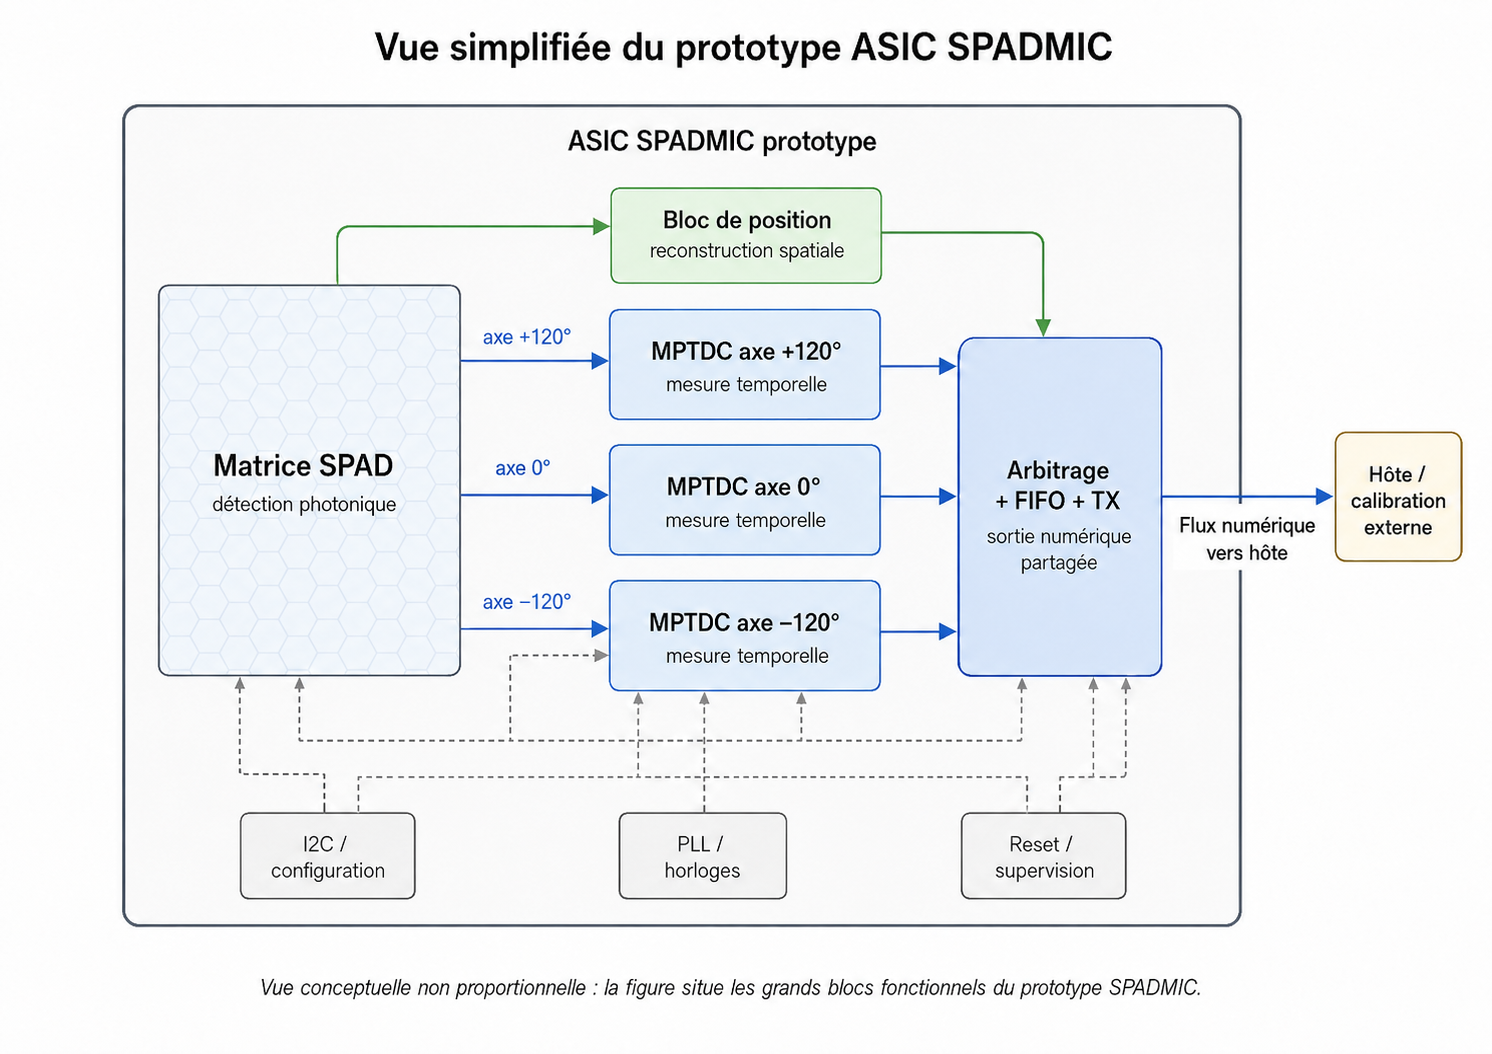
\includegraphics[width=\linewidth,height=0.70\textheight,keepaspectratio,trim=0 105 0 0,clip]{spadmic_mind_model.png}
    \end{column}
    \begin{column}{0.30\textwidth}
      \vspace{1.05cm}
      \small
      \begin{itemize}
        \item Prototype ASIC de lecture pour matrice SPAD
        \item Mesure temporelle fine associée aux événements détectés
      \end{itemize}
    \end{column}
  \end{columns}

  \takeaway{Le projet vise une mesure temporelle exploitable au sein de la chaîne de lecture SPADMIC.}
  \note{Objectif : introduire le projet sans entrer dans les détails du Vernier, de la CDC, de la trame ou de la calibration. À dire : la matrice SPAD détecte des événements, la mesure temporelle donne une information complémentaire, et le travail réalisé porte sur le cœur MPTDC, sa vérification et sa calibration pré-silicium. Transition : rendre concret le besoin temporel au niveau de la matrice SPAD.}
\end{frame}

% ---------------------------------------------------------------------------
\section[Besoin TDC]{Besoin système et choix d'architecture}

\chaptertransition{III}{Besoin système et choix d'architecture}{Introduire le TDC, ses métriques et la limite d'une mesure basée sur l'horloge système.}

\begin{frame}
  \frametitle{III. Qu'est-ce qu'un TDC ?}
  \lead{Un convertisseur temps-numérique transforme une information temporelle en donnée exploitable.}

  \vspace{0.12cm}
  \begin{center}
  \begin{tikzpicture}[
    x=1cm,y=1cm,
    pulse/.style={line width=1.05pt},
    lab/.style={font=\scriptsize\bfseries,text=navy2},
    block/.style={accentbox,minimum width=2.55cm,minimum height=1.05cm,font=\bfseries},
    outputbox/.style={mutedbox,minimum width=3.05cm,minimum height=0.96cm,font=\small\bfseries}
  ]
    \draw[time] (0,2.52) -- (3.75,2.52);
    \draw[time] (0,1.42) -- (3.75,1.42);
    \node[lab,anchor=east] at (-0.10,2.52) {START};
    \node[lab,anchor=east] at (-0.10,1.42) {STOP};

    \draw[pulse,draw=navy] (0.65,2.52) -- (0.65,2.92) -- (1.00,2.92) -- (1.00,2.52);
    \draw[pulse,draw=amber] (2.82,1.42) -- (2.82,1.82) -- (3.17,1.82) -- (3.17,1.42);
    \draw[<->,draw=amber,line width=0.8pt] (0.82,0.78) -- node[below,font=\scriptsize] {intervalle $\Delta t$} (3.00,0.78);
    \draw[time,densely dashed] (0.82,0.92) -- (0.82,2.95);
    \draw[time,densely dashed] (3.00,0.92) -- (3.00,1.86);

    \node[block] (tdc) at (5.45,1.97) {TDC};
    \node[font=\scriptsize,text=muted] at (5.45,1.23) {temps $\rightarrow$ numérique};
    \node[outputbox] (code) at (8.95,1.97) {code numérique\\[-1pt]{\ttfamily 010110...}};

    \draw[arrow] (3.75,1.97) -- (tdc.west);
    \draw[arrow] (tdc.east) -- (code.west);
    \node[font=\scriptsize,text=muted,align=center] at (8.95,0.95) {donnée exploitable\\par la chaîne numérique};
  \end{tikzpicture}
  \end{center}

  \vspace{0.12cm}
  \small
  \begin{columns}[T,totalwidth=0.92\textwidth]
    \begin{column}{0.45\textwidth}
      \begin{itemize}
        \item Convertisseur temps-numérique
        \item Mesure un intervalle de temps
      \end{itemize}
    \end{column}
    \begin{column}{0.45\textwidth}
      \begin{itemize}
        \item Transforme le temps en donnée numérique
        \item Date finement les événements SPAD
      \end{itemize}
    \end{column}
  \end{columns}

  \takeaway{Le TDC fait le lien entre un événement asynchrone et une donnée temporelle exploitable.}
  \note{Objectif : poser la définition avant les compromis. À dire : un TDC convertit un temps ou un intervalle START/STOP en un code numérique. Dans SPADMIC, il sert à dater finement les impulsions issues de la matrice SPAD. Transition : une fois ce rôle compris, expliquer les exigences du système.}
\end{frame}

% ---------------------------------------------------------------------------
\begin{frame}
  \frametitle{III. Exigences principales pour notre TDC}
  \lead{Le choix d'architecture vient d'un ensemble de besoins de mesure et de contraintes ASIC.}

  \vspace{0.20cm}
  \begin{columns}[T,totalwidth=0.94\textwidth]
    \begin{column}{0.45\textwidth}
      {\bfseries\color{navy2}Besoins fonctionnels}
      \vspace{0.08cm}
      {\color{line}\rule{\linewidth}{0.35pt}}
      \small
      \begin{itemize}
        \item Préserver l'instant d'arrivée des événements
        \item Transformer une information temporelle en donnée numérique
        \item Conserver assez d'information pour reconstruire la mesure
        \item Rester compatible avec des événements rapides et asynchrones
      \end{itemize}
    \end{column}
    \begin{column}{0.04\textwidth}
      \centering
      \vspace{0.14cm}
      {\color{line!70}\rule{0.35pt}{3.02cm}}
    \end{column}
    \begin{column}{0.45\textwidth}
      {\bfseries\color{navy2}Contraintes d'intégration}
      \vspace{0.08cm}
      {\color{line}\rule{\linewidth}{0.35pt}}
      \small
      \begin{itemize}
        \item Implémentation réaliste dans un ASIC
        \item Lecture compacte et exploitable
        \item Consommation et surface maîtrisées
        \item Calibration possible hors circuit
      \end{itemize}
    \end{column}
  \end{columns}

  \vspace{0.26cm}
  \begin{center}
    \begin{tikzpicture}
      \node[warnbox,minimum width=0.82\textwidth,text width=0.76\textwidth,align=center,font=\small]
        {\textbf{Compromis} central : préserver la finesse temporelle sans rendre la lecture, la calibration ou l'intégration irréalistes};
    \end{tikzpicture}
  \end{center}

  \takeaway{La résolution nominale n'a de sens que si la mesure peut être lue, vérifiée et corrigée.}
  \note{Objectif : structurer les besoins avant les métriques. À dire : l'architecture n'est pas choisie uniquement pour gagner en résolution ; elle doit rester intégrable, observable et compatible avec le débit et le réarmement. Transition : définir les métriques qui permettent d'évaluer ces exigences.}
\end{frame}

% ---------------------------------------------------------------------------
\begin{frame}
  \frametitle{III. Métriques clés d'un TDC}
  \lead{Quelques grandeurs permettent de lire le comportement temporel, linéaire et statistique d'un TDC.}

  \vspace{0.02cm}
  \begin{columns}[T,totalwidth=0.98\textwidth]
    \begin{column}{0.55\textwidth}
      \centering
      \begin{tikzpicture}[x=1cm,y=1cm]
        \def\w{6.45}
        \def\c{2.22}
        \def\rh{0.62}
        \fill[navy2] (0,3.10) rectangle (\w,3.72);
        \node[anchor=west,font=\scriptsize\bfseries,text=white] at (0.20,3.41) {Métrique};
        \node[anchor=west,font=\scriptsize\bfseries,text=white] at (\c+0.20,3.41) {Lecture physique};
        \draw[white!45,line width=0.35pt] (\c,3.18) -- (\c,3.64);

        \foreach \y/\bg in {2.48/navy2!8,1.86/soft,1.24/navy2!8,0.62/soft,0/navy2!8} {
          \fill[\bg] (0,\y) rectangle (\w,\y+\rh);
          \draw[white,line width=0.35pt] (0,\y) -- (\w,\y);
        }
        \draw[draw=line,line width=0.45pt] (0,0) rectangle (\w,3.72);
        \draw[draw=line,line width=0.35pt] (\c,0) -- (\c,3.72);

        \node[anchor=west,font=\scriptsize\bfseries,text=navy2] at (0.20,2.79) {Résolution / LSB};
        \node[anchor=west,text width=3.78cm,align=left,font=\scriptsize] at (\c+0.20,2.79) {largeur minimale d'un pas\\temporel};

        \node[anchor=west,font=\scriptsize\bfseries,text=navy2] at (0.20,2.17) {Plage dynamique};
        \node[anchor=west,text width=3.78cm,align=left,font=\scriptsize] at (\c+0.20,2.17) {intervalle mesurable avant\\saturation};

        \node[anchor=west,font=\scriptsize\bfseries,text=navy2] at (0.20,1.55) {DNL};
        \node[anchor=west,text width=3.78cm,align=left,font=\scriptsize] at (\c+0.20,1.55) {écart local de largeur d'un palier};

        \node[anchor=west,font=\scriptsize\bfseries,text=navy2] at (0.20,0.93) {INL};
        \node[anchor=west,text width=3.78cm,align=left,font=\scriptsize] at (\c+0.20,0.93) {dérive cumulée face à la\\réponse idéale};

        \node[anchor=west,font=\scriptsize\bfseries,text=navy2] at (0.20,0.31) {Précision RMS};
        \node[anchor=west,text width=3.78cm,align=left,font=\scriptsize] at (\c+0.20,0.31) {dispersion de l'erreur reconstruite};
      \end{tikzpicture}%
    \end{column}
    \begin{column}{0.39\textwidth}
      \centering
      \vspace{0.05cm}
      \resizebox{\linewidth}{!}{%
      \begin{tikzpicture}[x=0.70cm,y=0.62cm]
        \draw[->,draw=ink!70,line width=0.65pt] (0,0) -- (6.75,0);
        \draw[->,draw=ink!70,line width=0.65pt] (0,0) -- (0,4.86);
        \node[font=\scriptsize,anchor=north east,text=muted] at (6.62,-0.24) {temps};
        \node[font=\scriptsize,anchor=south,rotate=90,text=muted] at (-0.43,4.55) {code};

        \foreach \x in {1,2,3,4,5}
          \draw[draw=line,line width=0.28pt] (\x,0) -- (\x,4.12);
        \foreach \y in {1,2,3,4}
          \draw[draw=line,line width=0.28pt] (0,\y) -- (5.86,\y);

        \draw[draw=muted,dashed,line width=0.78pt]
          (0,0) -- (1,0) -- (1,1) -- (2,1) -- (2,2) -- (3,2)
          -- (3,3) -- (4,3) -- (4,4) -- (5,4);
        \draw[draw=navy,line width=1.18pt]
          (0,0) -- (0.74,0) -- (0.74,1) -- (2.20,1) -- (2.20,2)
          -- (3.08,2) -- (3.08,3) -- (4.46,3) -- (4.46,4) -- (5.38,4);

        \draw[<->,draw=navy,line width=0.78pt] (1.0,4.34) -- node[above,font=\scriptsize,text=navy] {LSB idéal} (2.0,4.34);
        \draw[<->,draw=amber,line width=0.85pt] (0.74,0.46) -- node[below,font=\scriptsize,text=amber] {DNL} (1.0,0.46);
        \draw[<->,draw=ink!70,line width=0.72pt] (4.0,3.32) -- node[right,font=\scriptsize,align=left] {INL\\cumulée} (4.46,3.32);
        \draw[<->,draw=navy2,line width=0.78pt] (0,-0.72) -- node[below,font=\scriptsize,align=center] {plage\\dynamique} (5.38,-0.72);
        \node[font=\scriptsize\bfseries,text=navy2,align=center] at (3.12,4.96) {Fonction de transfert\\non idéale};
      \end{tikzpicture}%
      }
    \end{column}
  \end{columns}

  \vspace{0.16cm}
  \begin{center}
    \small\color{muted}Une bonne résolution ne garantit pas, à elle seule, une précision temporelle faible
  \end{center}

  \takeaway{Le support doit défendre un système de mesure, pas une formule isolée.}
  \note{Objectif : donner au jury les critères de lecture des résultats. À dire : la résolution correspond au pas, la plage à l'intervalle utile, la DNL aux écarts locaux et l'INL à la dérive cumulée. Le RMS sera utilisé plus tard pour quantifier l'erreur après reconstruction et calibration. Transition : descendre vers les paramètres concrets du MPTDC.}
\end{frame}

% ---------------------------------------------------------------------------
\begin{frame}
  \frametitle{III. Cahier des charges du MPTDC}
  \lead{Les objectifs de mesure doivent rester compatibles avec les contraintes d'intégration ASIC.}

  \vspace{0.12cm}
  \begin{center}
  \begin{tikzpicture}[x=1cm,y=1cm]
    \def\w{9.20}
    \def\c{4.72}
    \def\rh{0.48}
    \def\top{4.34}
    \fill[navy2] (0,\top) rectangle (\w,\top+\rh);
    \node[anchor=west,font=\scriptsize\bfseries,text=white] at (0.24,\top+0.24) {Paramètre};
    \node[anchor=west,font=\scriptsize\bfseries,text=white] at (\c+0.24,\top+0.24) {Valeur / cible};
    \draw[white!50,line width=0.35pt] (\c,\top+0.08) -- (\c,\top+\rh-0.08);

    \foreach \i/\bg in {0/navy2!6,1/soft,2/navy2!6,3/soft,4/navy2!6,5/soft,6/navy2!6,7/soft} {
      \pgfmathsetmacro{\y}{\top-(\i+1)*\rh}
      \fill[\bg] (0,\y) rectangle (\w,\y+\rh);
      \draw[white,line width=0.35pt] (0,\y) -- (\w,\y);
    }
    \draw[draw=line,line width=0.45pt] (0,\top-8*\rh) rectangle (\w,\top+\rh);
    \draw[draw=line,line width=0.35pt] (\c,\top-8*\rh) -- (\c,\top+\rh);

    \node[anchor=west,font=\scriptsize\bfseries,text=navy2] at (0.24,4.10) {Résolution temporelle LSB};
    \node[anchor=west,font=\scriptsize] at (\c+0.24,4.10) {10 ps};
    \node[anchor=west,font=\scriptsize\bfseries,text=navy2] at (0.24,3.62) {DNL};
    \node[anchor=west,font=\scriptsize] at (\c+0.24,3.62) {$< 1$ LSB};
    \node[anchor=west,font=\scriptsize\bfseries,text=navy2] at (0.24,3.14) {INL};
    \node[anchor=west,font=\scriptsize] at (\c+0.24,3.14) {$< 1$ LSB};
    \node[anchor=west,font=\scriptsize\bfseries,text=navy2] at (0.24,2.66) {Horloge système};
    \node[anchor=west,font=\scriptsize] at (\c+0.24,2.66) {160 MHz};
    \node[anchor=west,font=\scriptsize\bfseries,text=navy2] at (0.24,2.18) {Surface totale estimée de l'ASIC};
    \node[anchor=west,font=\scriptsize] at (\c+0.24,2.18) {$\sim 10$ mm$^2$};
    \node[anchor=west,font=\scriptsize\bfseries,text=navy2] at (0.24,1.70) {Surface estimée du MPTDC};
    \node[anchor=west,font=\scriptsize] at (\c+0.24,1.70) {$\sim 1$ mm$^2$};
    \node[anchor=west,font=\scriptsize\bfseries,text=navy2] at (0.24,1.22) {Sortie numérique};
    \node[anchor=west,font=\scriptsize] at (\c+0.24,1.22) {16 bits DDR};
    \node[anchor=west,font=\scriptsize\bfseries,text=navy2] at (0.24,0.74) {Méthode de calibration};
    \node[anchor=west,font=\scriptsize] at (\c+0.24,0.74) {calibration externe pour cette version};
  \end{tikzpicture}
  \end{center}

  \vspace{0.08cm}
  \begin{center}
    \small\color{muted}Objectif : concilier finesse temporelle, intégration ASIC et calibration externe
  \end{center}

  \takeaway{Le MPTDC doit respecter simultanément des cibles temporelles, numériques et physiques.}
  \note{Objectif : poser le cahier des charges avant d'expliquer la limite de l'horloge système. À dire : le bloc ne peut pas être jugé uniquement sur un pas temporel ; il doit aussi tenir la surface, la sortie DDR 16 bits et la stratégie de calibration externe. Transition : montrer pourquoi l'horloge système seule ne peut pas porter cette finesse.}
\end{frame}

% ---------------------------------------------------------------------------
\begin{frame}
  \frametitle{III. Pourquoi l'horloge système ne suffit pas ?}
  \lead{L'horloge système pilote la lecture ; elle ne doit pas définir le pas temporel fin.}

  \vspace{-0.02cm}
  \begin{center}
  \begin{tikzpicture}[x=0.98cm,y=0.84cm]
    \draw[time] (0.4,3.0) -- (9.2,3.0);
    \node[font=\scriptsize\bfseries,text=navy2,anchor=east] at (0.22,3.0) {horloge};
    \foreach \x in {1.0,2.9,4.8,6.7,8.6} {
      \draw[draw=navy,line width=1.0pt] (\x,2.66) -- (\x,3.34);
      \draw[draw=line,line width=0.35pt] (\x,0.85) -- (\x,3.45);
    }
    \draw[<->,draw=navy,line width=0.75pt] (1.0,3.62) -- node[above,font=\scriptsize] {$T_{\mathrm{clk}}\approx6{,}25$ ns} (2.9,3.62);

    \draw[time] (0.4,1.78) -- (9.2,1.78);
    \node[font=\scriptsize\bfseries,text=navy2,anchor=east] at (0.22,1.78) {événement};
    \draw[draw=amber,line width=1.05pt] (2.18,1.78) -- (2.18,2.20) -- (2.48,2.20) -- (2.48,1.78);
    \node[font=\scriptsize,text=amber,anchor=south] at (2.33,2.24) {asynchrone};

    \draw[softarrow,draw=muted] (2.48,1.56) -- (2.90,1.56);
    \draw[<->,draw=amber,line width=0.85pt] (2.33,1.07) -- node[below,font=\scriptsize,align=center,text=amber] {erreur de\\quantification} (2.90,1.07);
    \draw[draw=amber,densely dashed,line width=0.65pt] (2.33,1.02) -- (2.33,2.25);
    \draw[draw=amber,densely dashed,line width=0.65pt] (2.90,1.02) -- (2.90,3.32);
    \node[warnbox,minimum width=2.65cm,minimum height=0.92cm,font=\scriptsize,align=center] at (7.05,1.65)
      {Attendre le prochain front\\détruit l'information fine};
  \end{tikzpicture}
  \end{center}

  \vspace{-0.02cm}
  \small
  \begin{columns}[T,totalwidth=0.92\textwidth]
    \begin{column}{0.46\textwidth}
      \begin{itemize}
        \item Les événements SPAD sont asynchrones
        \item Ils n'arrivent pas alignés sur l'horloge système
      \end{itemize}
    \end{column}
    \begin{column}{0.46\textwidth}
      \begin{itemize}
        \item À 160 MHz, la période vaut environ 6,25 ns
        \item Attendre le prochain front détruit l'information temporelle fine
        \item Il faut une mesure locale plus fine
      \end{itemize}
    \end{column}
  \end{columns}

  \vspace{-0.02cm}
  \begin{center}
    \smalltag{navy}{Ce besoin motive le principe Vernier}
  \end{center}

  \takeaway{D'où l'intérêt d'une architecture Vernier déclenchée localement par les événements.}
  \note{Objectif : justifier l'asynchrone avant d'entrer dans le Vernier. À dire : l'horloge système reste utile pour piloter et lire, mais elle imposerait une granularité d'environ 6,25 ns si elle servait directement à dater les événements. Transition : introduire le Vernier comme moyen de créer une finesse temporelle locale.}
\end{frame}

% ---------------------------------------------------------------------------
\section[Arch. MPTDC]{Architecture MPTDC}

\chaptertransition{IV}{Architecture MPTDC}{Passer du besoin de mesure au principe Vernier puis au bloc intégré dans SPADMIC.}

\begin{frame}
  \frametitle{IV. Principe Vernier monophase}
  \lead{Deux oscillateurs proches convertissent un intervalle START/STOP en rattrapage mesurable.}

  \vspace{0.02cm}
  \begin{center}
      \resizebox{0.95\textwidth}{!}{%
      \begin{tikzpicture}[
        x=1.0cm,y=0.64cm,
        sig/.style={font=\scriptsize\bfseries,anchor=east,text=navy2},
        wave/.style={line width=0.9pt,draw=ink},
        slow/.style={line width=1.05pt,draw=navy},
        fast/.style={line width=1.05pt,draw=amber},
        guide/.style={densely dashed,line width=0.55pt,draw=muted},
        cnt/.style={draw=line,fill=white,rounded corners=1pt,minimum height=0.38cm,font=\tiny,align=center},
        event/.style={font=\tiny\bfseries,text=muted}
      ]
        \fill[amberSoft] (6.44,0.34) rectangle (6.78,6.63);

        \foreach \y in {6.10,5.25,4.20,3.25,2.08,1.25,0.44}
          \draw[time] (1.34,\y) -- (8.62,\y);

        \node[sig] at (1.12,6.10) {START};
        \node[sig] at (1.12,5.25) {STOP};
        \node[sig] at (1.12,4.20) {osc. lent};
        \node[sig] at (1.12,3.25) {osc. rapide};
        \node[sig] at (1.12,2.08) {compteur lent};
        \node[sig] at (1.12,1.25) {compteur rapide};
        \node[sig] at (1.12,0.44) {coïncidence};

        \draw[guide] (1.72,0.20) -- (1.72,6.72);
        \draw[guide] (2.44,0.20) -- (2.44,6.72);
        \draw[guide,draw=amber] (6.60,0.20) -- (6.60,6.72);
        \node[event,anchor=south] at (1.72,6.76) {START};
        \node[event,anchor=south] at (2.44,6.76) {STOP};
        \node[event,anchor=south,text=amber] at (6.60,6.76) {coïncidence};

        \draw[wave] (1.34,6.10) -- (1.61,6.10) -- (1.61,6.45) -- (1.84,6.45) -- (1.84,6.10) -- (8.62,6.10);
        \draw[wave] (1.34,5.25) -- (2.33,5.25) -- (2.33,5.60) -- (2.56,5.60) -- (2.56,5.25) -- (8.62,5.25);

        \foreach \x/\lab in {1.72/$S_0$,3.34/$S_1$,4.96/$S_2$,6.60/$S_3$} {
          \draw[slow] (\x,4.20) -- (\x,4.55) -- (\x+0.20,4.55) -- (\x+0.20,4.20);
          \node[font=\tiny,text=navy] at (\x+0.10,4.78) {\lab};
        }
        \foreach \x/\lab in {2.44/$F_0$,3.84/$F_1$,5.18/$F_2$,6.60/$F_3$} {
          \draw[fast] (\x,3.25) -- (\x,3.60) -- (\x+0.20,3.60) -- (\x+0.20,3.25);
          \node[font=\tiny,text=amber] at (\x+0.10,3.83) {\lab};
        }

        \draw[<->,draw=navy,line width=0.70pt] (1.72,3.92) -- node[above,font=\tiny,text=navy] {$T_{\mathrm{slow}}$} (3.34,3.92);
        \draw[<->,draw=amber,line width=0.70pt] (2.44,2.93) -- node[below,font=\tiny,text=amber] {$T_{\mathrm{fast}}$} (3.84,2.93);
        \draw[<->,draw=muted,line width=0.55pt] (3.34,4.66) -- (3.84,4.66);
        \node[font=\tiny,text=muted,anchor=west] at (4.02,5.02) {écart qui diminue};

        \node[cnt,minimum width=1.22cm] at (2.50,2.08) {$N_s=0$};
        \node[cnt,minimum width=1.22cm] at (4.14,2.08) {$N_s=1$};
        \node[cnt,minimum width=1.22cm] at (5.76,2.08) {$N_s=2$};
        \node[cnt,minimum width=0.86cm,draw=navy!55,fill=navy!5] at (7.25,2.08) {gelé};

        \node[cnt,minimum width=1.22cm] at (3.14,1.25) {$N_f=0$};
        \node[cnt,minimum width=1.22cm] at (4.54,1.25) {$N_f=1$};
        \node[cnt,minimum width=1.22cm] at (5.92,1.25) {$N_f=2$};
        \node[cnt,minimum width=0.86cm,draw=amber!65,fill=amberSoft] at (7.25,1.25) {gelé};

        \draw[fast] (6.60,0.44) -- (6.60,0.78) -- (6.82,0.78) -- (6.82,0.44);
        \node[font=\tiny\bfseries,text=amber,anchor=west] at (6.94,0.67) {fin de mesure};
      \end{tikzpicture}%
      }
  \end{center}

  \takeaway{Le Vernier transforme une petite différence physique en information temporelle fine.}
  \note{Objectif : expliquer le mécanisme au tableau avec un vrai chronogramme monophase. À dire : START lance l'oscillateur lent, STOP lance l'oscillateur rapide, le rapide a une période plus courte et réduit l'écart jusqu'à la coïncidence. Les compteurs donnent la partie grossière, la coïncidence déclenche le reset ou la fin de mesure. Transition : expliquer pourquoi l'observation multiphase enrichit ce principe.}
\end{frame}

% ---------------------------------------------------------------------------
\begin{frame}
  \frametitle{IV. Principe Vernier multiphase pour SPADMIC}

  \vspace{-0.02cm}
  \begin{columns}[T,totalwidth=0.99\textwidth]
    \begin{column}{0.74\textwidth}
      \centering
      \resizebox{\linewidth}{!}{%
      \begin{tikzpicture}[
        x=1cm,y=1cm,
        input/.style={font=\scriptsize\bfseries,text=navy2,anchor=east},
        front/.style={basebox,minimum width=1.25cm,minimum height=1.10cm,font=\scriptsize\bfseries,align=center},
        matrix/.style={basebox,minimum width=1.78cm,minimum height=2.18cm,font=\scriptsize\bfseries,align=center},
        cnt/.style={basebox,minimum width=1.42cm,minimum height=0.54cm,font=\scriptsize\bfseries,align=center},
        obs/.style={accentbox,minimum width=1.58cm,minimum height=1.02cm,font=\scriptsize\bfseries,align=center},
        tx/.style={basebox,draw=navy!60,fill=navy!5,minimum width=1.38cm,minimum height=0.78cm,font=\scriptsize\bfseries,align=center},
        tap/.style={font=\tiny\bfseries,align=center},
        invslow/.style={draw=amber!82!black,fill=white,line width=0.75pt},
        invfast/.style={draw=navy!82!black,fill=white,line width=0.75pt}
      ]
        \node[input] (start) at (-0.08,3.24) {START};
        \node[input] (stop) at (-0.08,2.36) {STOP};
        \node[front] (pre) at (0.80,2.80) {Prélogique\\front-end};

        \draw[arrow,draw=ink!65] (start.east) -- ([yshift=0.22cm]pre.west);
        \draw[arrow,draw=ink!65] (stop.east) -- ([yshift=-0.22cm]pre.west);

        \node[font=\scriptsize\bfseries,text=amber!82!black] at (3.34,5.02) {Oscillateur lent};
        \node[font=\scriptsize\bfseries,text=navy!82!black] at (3.34,0.98) {Oscillateur rapide};

        \draw[arrow,draw=amber!78!black] ([yshift=0.22cm]pre.east) -- (1.64,4.20);
        \draw[arrow,draw=navy!78!black] ([yshift=-0.22cm]pre.east) -- (1.64,1.80);

        \foreach \i/\lab in {0/S1,1/S2,2/S3,3/S4,4/S5} {
          \pgfmathsetmacro{\x}{1.72+0.72*\i}
          \draw[invslow] (\x,4.00) -- (\x,4.40) -- (\x+0.39,4.20) -- cycle;
          \draw[invslow] (\x+0.44,4.20) circle (0.045);
          \draw[amber!78!black,line width=0.70pt] (\x+0.49,4.20) -- (\x+0.70,4.20);
          \draw[amber!70!black,line width=0.55pt] (\x+0.49,4.20) -- (\x+0.49,4.58);
          \node[tap,text=amber!82!black] at (\x+0.49,4.72) {\lab};
        }
        \foreach \i/\lab in {0/F1,1/F2,2/F3,3/F4,4/F5} {
          \pgfmathsetmacro{\x}{1.72+0.72*\i}
          \draw[invfast] (\x,1.60) -- (\x,2.00) -- (\x+0.39,1.80) -- cycle;
          \draw[invfast] (\x+0.44,1.80) circle (0.045);
          \draw[navy!78!black,line width=0.70pt] (\x+0.49,1.80) -- (\x+0.70,1.80);
          \draw[navy!70!black,line width=0.55pt] (\x+0.49,1.80) -- (\x+0.49,1.42);
          \node[tap,text=navy!82!black] at (\x+0.49,1.27) {\lab};
        }

        \draw[amber!72!black,line width=0.90pt] (2.21,4.58) -- (5.20,4.58) -- (5.20,3.88) -- (5.92,3.88);
        \draw[navy!72!black,line width=0.90pt] (2.21,1.42) -- (5.20,1.42) -- (5.20,2.44) -- (5.92,2.44);

        \node[matrix] (pd) at (6.78,3.16) {};
        \node[font=\scriptsize\bfseries,text=navy2,align=center] at (6.78,3.73) {Matrice de phase\\$8\times8$};
        \begin{scope}[shift={(6.20,2.38)},x=0.155cm,y=0.155cm]
          \foreach \m in {0,...,7} {
            \foreach \n in {0,...,7} {
              \fill[white] (\m,\n) rectangle ++(0.78,0.78);
              \draw[line width=0.14pt,draw=line] (\m,\n) rectangle ++(0.78,0.78);
            }
          }
          \fill[amber!42] (1,5) rectangle ++(0.78,0.78);
          \fill[navy!30] (3,3) rectangle ++(0.78,0.78);
          \fill[amber!42] (6,1) rectangle ++(0.78,0.78);
        \end{scope}

        \node[cnt,draw=amber!70,fill=amberSoft] (cs) at (8.38,4.22) {Compteur lent};
        \node[cnt,draw=navy!62,fill=navy!5] (cf) at (8.38,1.86) {Compteur rapide};
        \node[obs,minimum width=1.82cm,minimum height=1.08cm] (obs) at (9.84,3.10) {Observables\\[-1pt]\scriptsize $N_s,N_f$\\[-1pt]\scriptsize $n_s,n_f,PD_{ij}$};
        \node[tx] (read) at (11.34,3.10) {export\\lecture};

        \draw[softarrow,draw=amber!75!black] (4.97,4.20) -- (cs.west);
        \draw[softarrow,draw=navy!75!black] (4.97,1.80) -- (cf.west);
        \draw[arrow,draw=ink!70] (pd.east) -- (obs.west);
        \draw[softarrow] (cs.east) -- ++(0.34,0) |- ([yshift=0.24cm]obs.west);
        \draw[softarrow] (cf.east) -- ++(0.34,0) |- ([yshift=-0.24cm]obs.west);
        \draw[arrow] (obs.east) -- node[above,font=\tiny\bfseries,text=navy] {$\leq15$} (read.west);

        \node[basebox,draw=line,fill=soft,minimum width=3.12cm,minimum height=0.42cm,font=\scriptsize] at (3.50,0.42)
          {$T_{\mathrm{LSB}} = T_{\mathrm{slow}} - T_{\mathrm{fast}}$};
      \end{tikzpicture}%
      }
    \end{column}
    \begin{column}{0.24\textwidth}
      \vspace{0.38cm}
      \footnotesize
      \begin{itemize}
        \item Pas fin subdivisé : $\Delta = T_{\mathrm{LSB}}/N_e$
        \item Plusieurs observables pour un même événement
        \item Jusqu'à 15 mesures exportées par conversion dans SPADMIC
        \item Combinaison statistique externe : gain $\sim 1/\sqrt{N}$
      \end{itemize}
    \end{column}
  \end{columns}

  \takeaway{Le multiphase relie phases, compteurs et matrice 8x8 pour exporter plusieurs observables calibrables.}
  \note{Objectif : montrer l'architecture multiphase dans le contexte SPADMIC. À dire : START et STOP alimentent une prélogique, deux oscillateurs génèrent des phases lentes et rapides, la matrice 8x8 détecte les couples de phase et les compteurs complètent les observables exportés. Transition : lire ce principe dans un chronogramme.}
\end{frame}

% ---------------------------------------------------------------------------
\begin{frame}
  \frametitle{IV. Chronogramme du Vernier multiphase}

  \vspace{-0.03cm}
  \begin{center}
    \resizebox{0.985\textwidth}{0.70\textheight}{%
    \begin{tikzpicture}[
      x=1cm,y=1cm,
      lab/.style={font=\scriptsize\bfseries,anchor=east,text=navy2},
      grouplab/.style={font=\scriptsize\bfseries,anchor=east,text=muted},
      wave/.style={line width=0.82pt,line cap=round,line join=round},
      base/.style={line width=0.28pt,draw=line},
      slow/.style={wave,draw=amber!86!black},
      fast/.style={wave,draw=navy!86!black},
      startstop/.style={wave,draw=ink},
      guide/.style={densely dashed,line width=0.48pt,draw=muted!72},
      cntbox/.style={draw=line,fill=white,rounded corners=0.6pt,line width=0.35pt,font=\tiny\bfseries,text=navy2,align=center,inner sep=1.2pt},
      pulsepd/.style={line width=0.90pt,draw=ink!80,line cap=round,line join=round}
    ]
      \fill[amber!5] (1.74,3.54) rectangle (13.10,5.62);
      \fill[navy!4] (1.74,0.92) rectangle (13.10,3.00);
      \fill[soft] (1.74,-1.12) rectangle (13.10,0.54);

      \foreach \y in {6.70,6.10,5.36,5.00,4.64,4.28,3.92,3.36,2.74,2.38,2.02,1.66,1.30,0.74,0.18,-0.30,-0.66,-1.02} {
        \draw[base] (1.74,\y) -- (13.10,\y);
      }

      \node[lab] at (1.48,6.70) {START};
      \node[lab] at (1.48,6.10) {STOP};
      \node[grouplab] at (1.48,5.56) {lent};
      \node[grouplab] at (1.48,2.94) {rapide};
      \node[lab] at (1.48,3.36) {$N_{\mathrm{slow}}$};
      \node[lab] at (1.48,0.74) {$N_{\mathrm{fast}}$};
      \node[lab] at (1.48,0.18) {$n_s,n_f$};
      \node[lab] at (1.48,-0.30) {$PD_{1,4}$};
      \node[lab] at (1.48,-0.66) {$PD_{2,4}$};
      \node[lab] at (1.48,-1.02) {$PD_{3,5}$};

      \draw[startstop] (1.74,6.70) -- (2.04,6.70) -- (2.04,6.98) -- (2.38,6.98) -- (2.38,6.70) -- (13.10,6.70);
      \draw[startstop] (1.74,6.10) -- (3.06,6.10) -- (3.06,6.38) -- (3.40,6.38) -- (3.40,6.10) -- (13.10,6.10);
      \node[font=\tiny\bfseries,text=muted] at (2.55,6.48) {$T_{\mathrm{hit}}$};

      \foreach \k/\y in {1/5.36,2/5.00,3/4.64,4/4.28,5/3.92} {
        \node[lab,text=amber!86!black] at (1.67,\y) {$S_{\k}$};
        \foreach \b in {2.10,4.72,7.34,9.96,12.58} {
          \pgfmathsetmacro{\xs}{\b+0.15*(\k-1)}
          \draw[slow] (\xs,\y) -- (\xs,\y+0.22) -- (\xs+0.46,\y+0.22) -- (\xs+0.46,\y);
        }
      }

      \foreach \k/\y in {1/2.74,2/2.38,3/2.02,4/1.66,5/1.30} {
        \node[lab,text=navy!86!black] at (1.67,\y) {$F_{\k}$};
        \foreach \b in {3.12,5.56,8.00,10.44,12.88} {
          \pgfmathsetmacro{\xf}{\b+0.11*(\k-1)}
          \draw[fast] (\xf,\y) -- (\xf,\y+0.22) -- (\xf+0.46,\y+0.22) -- (\xf+0.46,\y);
        }
      }

      \draw[<->,draw=amber!80!black,line width=0.45pt] (2.10,5.72) -- node[above,font=\tiny,text=amber!85!black] {$\tau_s$} (2.25,5.72);
      \draw[<->,draw=navy!80!black,line width=0.45pt] (3.12,3.10) -- node[above,font=\tiny,text=navy!85!black] {$\tau_f$} (3.23,3.10);

      \foreach \xa/\xb/\txt in {2.10/4.72/0,4.72/7.34/1,7.34/9.96/2,9.96/12.58/3} {
        \draw[cntbox,fill=amber!7] (\xa,3.23) rectangle (\xb,3.49);
        \node[font=\tiny\bfseries,text=amber!85!black] at ({(\xa+\xb)/2},3.36) {\txt};
      }
      \foreach \xa/\xb/\txt in {3.12/5.56/0,5.56/8.00/1,8.00/10.44/2,10.44/12.88/3} {
        \draw[cntbox,fill=navy!6] (\xa,0.61) rectangle (\xb,0.87);
        \node[font=\tiny\bfseries,text=navy!85!black] at ({(\xa+\xb)/2},0.74) {\txt};
      }

      \foreach \x in {9.54,9.86,10.18} {
        \draw[guide] (\x,-1.20) -- (\x,6.96);
      }

      \foreach \xa/\xb/\txt in {8.92/9.54/2,9.54/9.86/3,9.86/10.18/4,10.18/10.82/5} {
        \draw[cntbox,fill=white] (\xa,0.05) rectangle (\xb,0.31);
        \node[font=\tiny\bfseries,text=navy2] at ({(\xa+\xb)/2},0.18) {\txt};
      }

      \draw[pulsepd] (1.74,-0.30) -- (9.54,-0.30) -- (9.54,-0.08) -- (9.76,-0.08) -- (9.76,-0.30) -- (13.10,-0.30);
      \draw[pulsepd] (1.74,-0.66) -- (9.86,-0.66) -- (9.86,-0.44) -- (10.08,-0.44) -- (10.08,-0.66) -- (13.10,-0.66);
      \draw[pulsepd] (1.74,-1.02) -- (10.18,-1.02) -- (10.18,-0.80) -- (10.40,-0.80) -- (10.40,-1.02) -- (13.10,-1.02);

    \end{tikzpicture}%
    }
  \end{center}

  \takeaway{Les phases et les compteurs produisent plusieurs observables temporels pour une même conversion.}
  \note{Objectif : montrer le comportement temporel multiphase sans répéter la motivation. À dire : les phases lentes et rapides évoluent en parallèle, les compteurs encadrent la mesure et quelques sorties PDij matérialisent des coïncidences exploitables. Transition : transformer cette observation en bloc MPTDC lisible et intégré dans SPADMIC.}
\end{frame}

% ---------------------------------------------------------------------------
\begin{frame}
  \frametitle{MPTDC : mesure locale, lecture système}
  \lead{Domaine de mesure Vernier d'un côté, domaine de lecture système de l'autre.}

  \begin{center}
    
\includegraphics[width=0.99\textwidth,height=0.73\textheight,keepaspectratio]{mptdc_block_diagram.pdf}
  \end{center}

  \takeaway{La séparation des domaines protège la finesse de mesure et organise la lecture.}
  \note{Objectif : montrer le choix d'ingénierie central du MPTDC. À dire : START/STOP lancent une mesure locale, puis l'horloge système récupère une image figée, contextualisée et sérialisée. Transition : zoomer sur la capture asynchrone.}
\end{frame}

% ---------------------------------------------------------------------------
\begin{frame}
  \frametitle{IV. START/STOP avant l'horloge système}
  \lead{Pas d'horloge système sur le chemin de lancement START/STOP.}

  \vspace{0.04cm}
  \begin{columns}[T,totalwidth=0.98\textwidth]
    \begin{column}{0.48\textwidth}
      \centering
      \resizebox{\linewidth}{!}{%
      \begin{tikzpicture}[
        node distance=0.34cm,
        blk/.style={basebox,minimum width=1.56cm,minimum height=0.56cm,font=\scriptsize},
        event/.style={font=\scriptsize\bfseries,text=navy2}
      ]
        \node[event] (st) {START};
        \node[blk,right=of st] (lst) {latch\\START};
        \node[blk,right=of lst,draw=navy!55,fill=navy!4] (sl) {anneau\\lent};
        \draw[arrow] (st) -- (lst);
        \draw[arrow] (lst) -- (sl);

        \node[event,below=0.70cm of st] (sp) {STOP};
        \node[blk,right=of sp] (lsp) {latch\\STOP};
        \node[blk,right=of lsp,draw=amber!65,fill=amberSoft] (fa) {anneau\\rapide};
        \draw[arrow] (sp) -- (lsp);
        \draw[arrow] (lsp) -- (fa);

        \node[warnbox,below=0.70cm of lsp,minimum width=4.48cm,align=center,font=\scriptsize] (msg)
          {Aucune reprise par l'horloge système\\avant le lancement de mesure};
        \draw[softarrow] (msg.north) -- (lsp.south);
      \end{tikzpicture}%
      }
    \end{column}
    \begin{column}{0.47\textwidth}
      \centering
      \resizebox{\linewidth}{!}{%
      \begin{tikzpicture}[
        x=0.88cm,y=0.55cm,
        lab/.style={font=\scriptsize\bfseries,anchor=east,text=navy2},
        wave/.style={line width=0.9pt,draw=ink},
        guide/.style={densely dashed,line width=0.55pt,draw=muted}
      ]
        \foreach \y in {4.70,3.85,2.80,1.95,0.88}
          \draw[time] (1.30,\y) -- (7.55,\y);
        \node[lab] at (1.08,4.70) {START};
        \node[lab] at (1.08,3.85) {latch S};
        \node[lab] at (1.08,2.80) {STOP};
        \node[lab] at (1.08,1.95) {latch F};
        \node[lab] at (1.08,0.88) {clear};

        \draw[guide] (1.72,0.55) -- (1.72,5.10);
        \draw[guide] (2.92,0.55) -- (2.92,5.10);
        \draw[guide,draw=amber] (6.44,0.55) -- (6.44,5.10);
        \node[font=\tiny\bfseries,text=muted] at (1.72,5.22) {front START};
        \node[font=\tiny\bfseries,text=muted] at (2.92,5.22) {front STOP};
        \node[font=\tiny\bfseries,text=amber] at (6.44,5.22) {clear};

        \draw[wave] (1.30,4.70) -- (1.62,4.70) -- (1.62,5.03) -- (1.84,5.03) -- (1.84,4.70) -- (7.55,4.70);
        \draw[wave,draw=navy] (1.30,3.85) -- (1.72,3.85) -- (1.72,4.18) -- (6.44,4.18) -- (6.44,3.85) -- (7.55,3.85);
        \draw[wave] (1.30,2.80) -- (2.82,2.80) -- (2.82,3.13) -- (3.04,3.13) -- (3.04,2.80) -- (7.55,2.80);
        \draw[wave,draw=amber] (1.30,1.95) -- (2.92,1.95) -- (2.92,2.28) -- (6.44,2.28) -- (6.44,1.95) -- (7.55,1.95);
        \draw[wave] (1.30,0.88) -- (6.32,0.88) -- (6.32,1.21) -- (6.56,1.21) -- (6.56,0.88) -- (7.55,0.88);
      \end{tikzpicture}%
      }
    \end{column}
  \end{columns}

  \takeaway{La capture asynchrone est un choix de mesure, pas une complication gratuite.}
  \note{Objectif : défendre la capture asynchrone. À dire : si START/STOP étaient d'abord repris par l'horloge système, celle-ci entrerait dans l'erreur de mesure. Transition : revenir aux observables de matrice qui devront être calibrées.}
\end{frame}

% ---------------------------------------------------------------------------
\begin{frame}
  \frametitle{IV. Matrice $8\times8$ : observables non uniformes}
  \lead{Les couples $(n_s,n_f)$ observés forment une répartition structurée, mais non uniforme.}

  \vspace{0.02cm}
  \begin{columns}[T,totalwidth=0.98\textwidth]
    \begin{column}{0.62\textwidth}
      \centering
      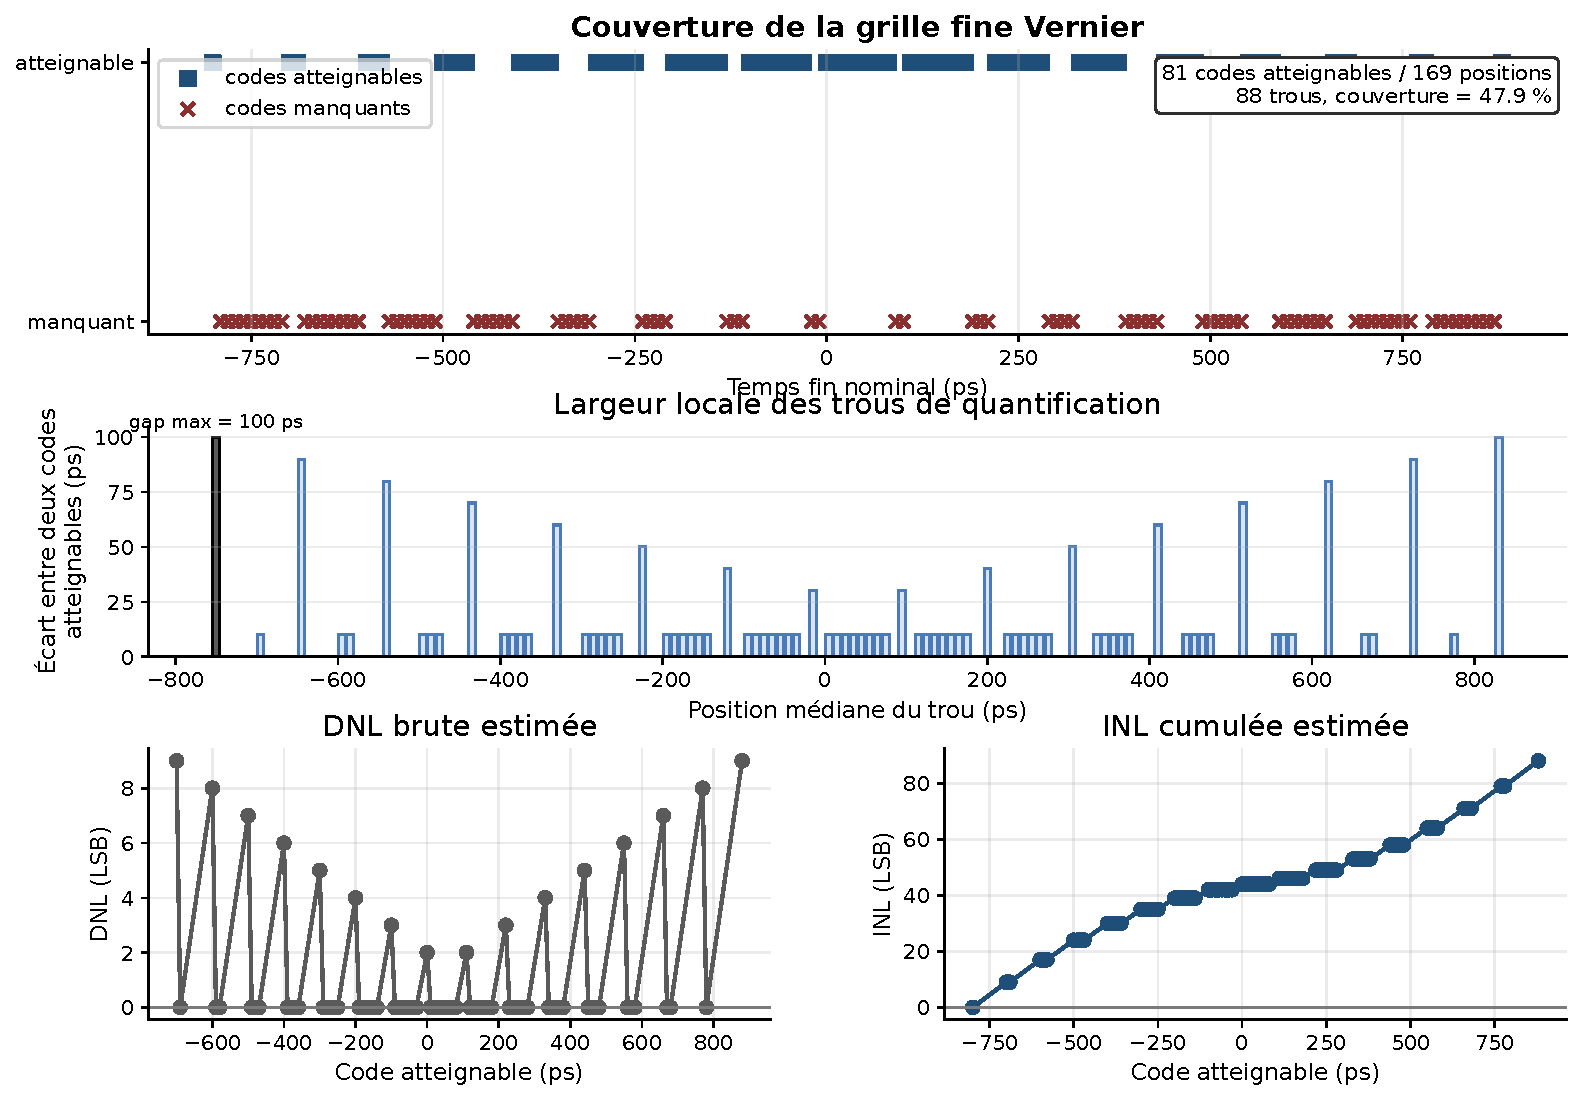
\includegraphics[width=\linewidth,height=0.66\textheight,keepaspectratio]{fine_grid_coverage.pdf}
      \vspace{-0.06cm}
      \smalltag{navy}{axes $n_s$ / $n_f$}\hspace{0.22cm}
      \smalltag{amber}{codes absents}
    \end{column}
    \begin{column}{0.32\textwidth}
      \vspace{0.22cm}
      \small
      \begin{itemize}
        \item 64 couples physiques observés
        \item Distribution temporelle non uniforme
        \item Certains codes sont absents
        \item Densité variable selon les couples
        \item Calibration externe nécessaire
      \end{itemize}
    \end{column}
  \end{columns}

  \takeaway{Le timestamp brut n'est pas le produit final : les observables exportées sont la matière de la calibration.}
  \note{Objectif : préparer la calibration sans la présenter comme une rustine. À dire : la matrice 8x8 donne 64 couples physiques, mais la distribution fine n'est pas uniforme ; certains codes peuvent être absents et plusieurs couples proches, donc le système exporte les observables plutôt qu'un timestamp final supposé uniforme. Transition : expliquer comment le protocole protège ces observables.}
\end{frame}

% ---------------------------------------------------------------------------
\begin{frame}
  \frametitle{IV. Snapshot avant clear}
  \lead{Snapshot, contexte, puis clear : l'image utile est protégée avant nettoyage.}

  \vspace{0.05cm}
  \begin{columns}[T,totalwidth=0.98\textwidth]
    \begin{column}{0.63\textwidth}
      \centering
      \resizebox{\linewidth}{!}{%
      \begin{tikzpicture}[
        node distance=0.28cm,
        stage/.style={basebox,minimum width=1.58cm,minimum height=0.62cm,font=\scriptsize},
        prot/.style={accentbox,minimum width=1.72cm,minimum height=0.62cm,font=\scriptsize}
      ]
        \node[stage] (hit) {mesure\\terminée};
        \node[prot,right=of hit] (snap) {snapshot};
        \node[prot,right=of snap] (ctx) {contexte\\écrit};
        \node[stage,right=of ctx,draw=amber!65,fill=amberSoft] (clear) {clear\\matrice};
        \node[stage,right=of clear] (read) {lecture\\TX};

        \draw[arrow] (hit) -- (snap);
        \draw[arrow] (snap) -- (ctx);
        \draw[arrow] (ctx) -- (clear);
        \draw[arrow] (clear) -- (read);

        \draw[navy,line width=0.9pt] ($(snap.south west)+(0,-0.28)$) -- node[below,font=\tiny\bfseries,text=navy] {information protégée} ($(ctx.south east)+(0,-0.28)$);
        \draw[amber,line width=0.9pt] ($(clear.south west)+(0,-0.28)$) -- node[below,font=\tiny\bfseries,text=amber] {front-end libéré} ($(clear.south east)+(0,-0.28)$);
      \end{tikzpicture}%
      }
    \end{column}
    \begin{column}{0.31\textwidth}
      \vspace{0.14cm}
      \small
      \begin{itemize}
        \item L'image utile est figée avant nettoyage
        \item Le clear intervient après écriture contexte
        \item Le reset global reste séparé du clear de conversion
        \item La trame lit un contexte stable
      \end{itemize}
    \end{column}
  \end{columns}

  \takeaway{Le clear n'est acceptable qu'après protection de l'information utile.}
  \note{Objectif : rendre mémorable la séquence snapshot, contexte, clear. À dire : on fige l'image, on l'écrit dans un contexte, puis seulement on nettoie ; le détail reset vs clear reste disponible en backup. Transition : montrer pourquoi deux contextes réduisent le temps mort.}
\end{frame}

% ---------------------------------------------------------------------------
\begin{frame}
  \frametitle{Deux contextes réduisent le temps mort}
  \lead{Deux contextes permettent de lire une image pendant que la suivante se prépare.}

  \begin{center}
    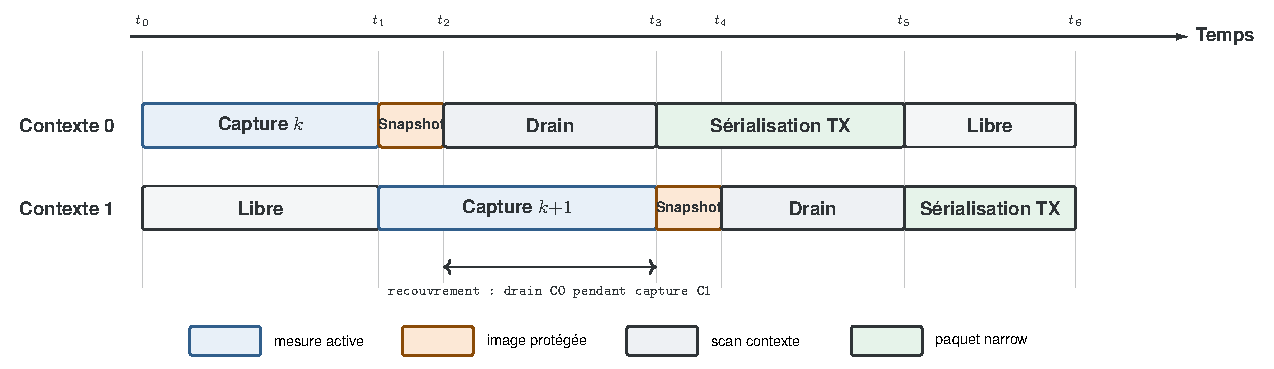
\includegraphics[width=0.98\textwidth,height=0.70\textheight,keepaspectratio]{context_pipeline.pdf}
  \end{center}

  \takeaway{Le double contexte réduit le temps mort lié à la lecture, mais reste une ressource bornée.}
  \note{Objectif : montrer le recouvrement capture / lecture. À dire : les contextes stockent des images de mesure, ils ne dupliquent pas la matrice Vernier. Transition : présenter la trame qui transporte ces observables hors du bloc.}
\end{frame}

% ---------------------------------------------------------------------------
\begin{frame}
  \frametitle{Trame 16 bit : observables}
  \lead{Format compact : META, HIT words, EOC, compteurs, phases et statuts.}

  \begin{center}
    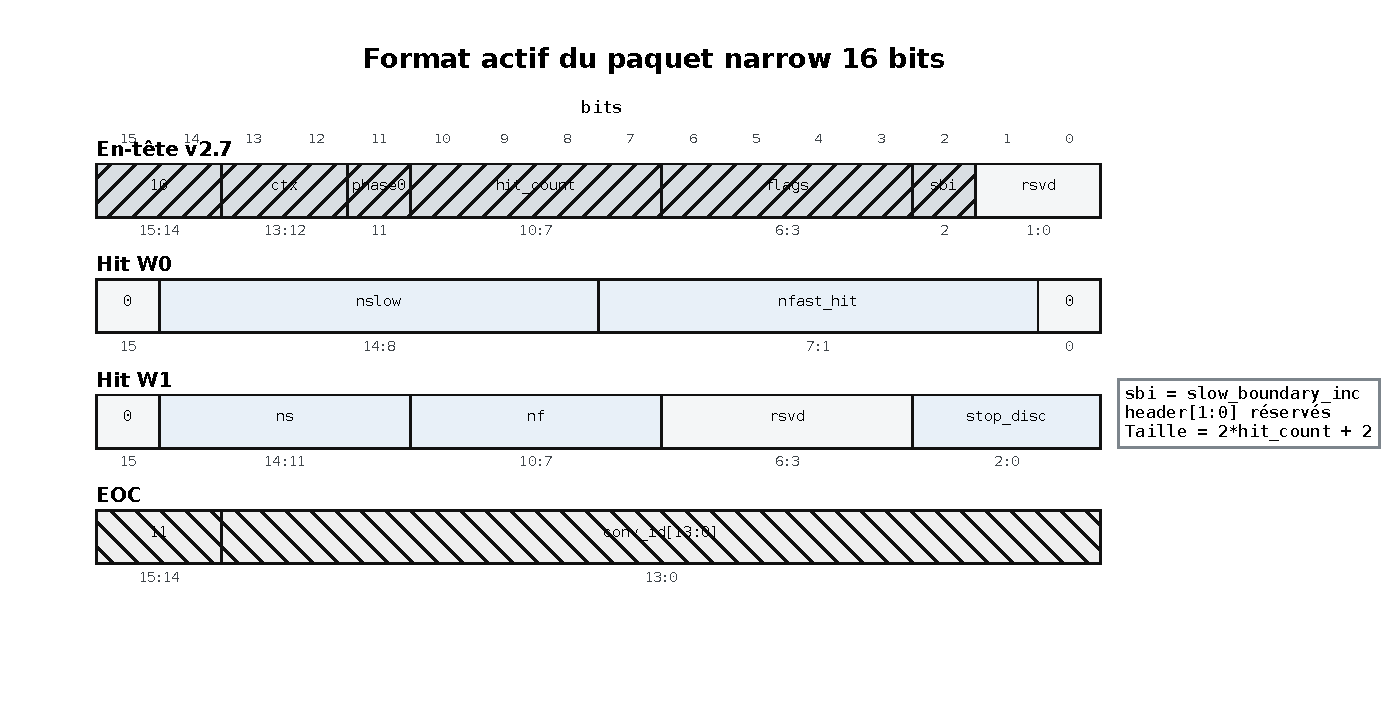
\includegraphics[width=0.96\textwidth,height=0.66\textheight,keepaspectratio]{packet_format_v27.pdf}
  \end{center}
  \vspace{-0.04cm}
  \centering
  \smalltag{navy}{16 bit}\hspace{0.35cm}
  \smalltag{navy}{$2N_{\mathrm{det}}+2$ mots}\hspace{0.35cm}
  \smalltag{navy}{$N_{\mathrm{det}}\leq15$}

  \takeaway{La compacité de sortie et la richesse d'observation sont deux contraintes simultanées.}
  \note{Objectif : expliquer le choix d'une sortie compacte. À dire : la trame 16 bit transporte les informations nécessaires à la LUT, pas seulement un temps final. Transition : justifier la calibration externe côté hôte.}
\end{frame}

\section[Vérification]{Vérification et calibration}

\chaptertransition{V}{Vérification et calibration}{Montrer comment le RTL est vérifié et comment les données brutes sont corrigées hors puce.}

% ---------------------------------------------------------------------------
\begin{frame}
  \frametitle{Calibration externe architecturale}
  \lead{Le silicium exporte une trame compacte ; la correction reste côté hôte.}

  \vspace{0.02cm}
  \begin{columns}[T,totalwidth=0.98\textwidth]
    \begin{column}{0.67\textwidth}
      \centering
      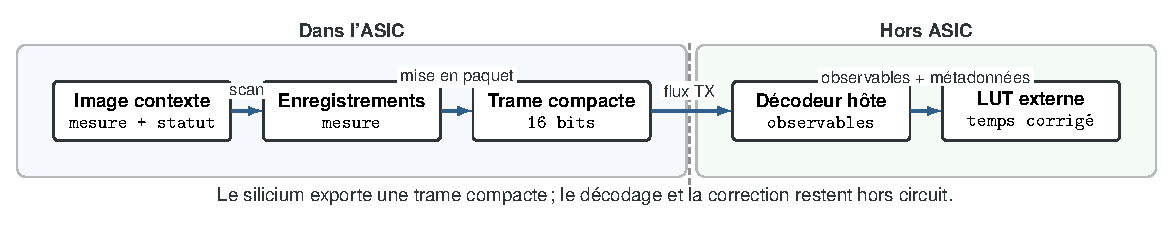
\includegraphics[width=\linewidth,height=0.68\textheight,keepaspectratio]{calibration_export_flow.pdf}
    \end{column}
    \begin{column}{0.29\textwidth}
      \vspace{0.18cm}
      \small
      \begin{itemize}
        \item Répartition des codes non uniforme
        \item Observables bruts insuffisants seuls
        \item Trame compacte exportée par l'ASIC
        \item Décodage et correction hors ASIC
        \item LUT externe vers temps corrigé
      \end{itemize}
    \end{column}
  \end{columns}

  \takeaway{La LUT n'est pas une rustine : elle fait partie du contrat d'observabilité.}
  \note{Objectif : défendre la LUT comme décision architecturale. À dire : l'ASIC reste compact et exporte les observables, tandis que le décodage et la correction restent côté hôte. La LUT transforme ces observables en temps corrigé. Transition : expliquer comment le RTL a été vérifié autour de ce contrat.}
\end{frame}

% ---------------------------------------------------------------------------
\begin{frame}
  \frametitle{V. Architecture du banc de vérification}
  \lead{La preuve utile porte sur les comportements qui peuvent casser une mesure : ordre, paquets, timeouts, rétropression.}

  \vspace{0.02cm}
  \begin{columns}[T,totalwidth=0.98\textwidth]
    \begin{column}{0.66\textwidth}
      \centering
      \begin{tikzpicture}[
        x=1cm,y=1cm,
        blk/.style={basebox,minimum width=1.42cm,minimum height=0.50cm,font=\scriptsize},
        smallblk/.style={basebox,minimum width=1.30cm,minimum height=0.44cm,font=\tiny},
        label/.style={font=\tiny\bfseries,text=muted,anchor=north west}
      ]
        \draw[rounded corners=2pt,draw=line,fill=white] (0.00,0.00) rectangle (7.70,4.65);
        \node[label] at (0.18,4.48) {TB\_top};

        \node[blk,draw=navy!55,fill=navy!4] (test) at (1.20,3.86) {Test};

        \draw[rounded corners=2pt,draw=line,fill=soft] (0.48,0.44) rectangle (6.28,3.38);
        \node[label,anchor=north east] at (6.10,3.22) {Env};

        \draw[rounded corners=2pt,draw=line,fill=white] (0.84,1.46) rectangle (4.30,3.02);
        \node[label] at (0.98,2.86) {Agent};

        \node[smallblk] (seq) at (1.62,2.38) {Sequencer};
        \node[smallblk] (drv) at (3.26,2.38) {Driver};
        \node[smallblk] (mon) at (3.26,1.62) {Monitor};
        \node[blk] (score) at (5.12,1.62) {Scoreboard};
        \node[smallblk,draw=navy!55,fill=navy!4] (ref) at (5.12,0.82) {modèle ref.};

        \node[blk] (iface) at (5.12,2.60) {Interface};
        \node[blk,draw=amber!65,fill=amberSoft] (dut) at (6.90,2.60) {DUT MPTDC};

        \draw[softarrow] (test.south) -- ++(0,-0.42) -| (seq.north);
        \draw[arrow] (seq.east) -- (drv.west);
        \draw[arrow] (drv) -- (iface);
        \draw[arrow] (iface) -- (dut);
        \draw[softarrow] (dut.south) -- ++(0,-1.15) -| (mon.south);
        \draw[softarrow] (mon.east) -- (score.west);
        \draw[softarrow] (ref) -- (score);

        \node[tinybox,minimum width=1.30cm] at (1.46,0.78) {paquets};
        \node[tinybox,minimum width=1.30cm] at (2.92,0.78) {watchdogs};
        \node[tinybox,minimum width=1.50cm] at (1.46,0.28) {rétropression};
        \node[tinybox,minimum width=1.30cm] at (2.92,0.28) {reset / clear};
      \end{tikzpicture}
    \end{column}
    \begin{column}{0.29\textwidth}
      \vspace{0.32cm}
      \small
      \begin{itemize}
        \item Stimuli dirigés et scénarios contraints
        \item Observation des sorties
        \item Comparaison au comportement attendu
        \item Vérification des paquets et cas limites
        \item Approche structurée inspirée des pratiques industrielles
      \end{itemize}
    \end{column}
  \end{columns}

  \takeaway{La vérification démontre un contrat numérique et protocolaire.}
  \note{Objectif : montrer la méthode de vérification sans prétendre au signoff complet. À dire : les scénarios ciblent les risques de protocole, puis monitors et scoreboard comparent les paquets attendus au modèle. Transition : clarifier précisément ce que cette vérification ne prouve pas.}
\end{frame}

% ---------------------------------------------------------------------------
\begin{frame}
  \frametitle{V. RTL $\neq$ signoff physique}
  \lead{Il faut dire exactement ce qui est validé, et ce qui reste hors preuve RTL.}

  \begin{columns}[T,totalwidth=\textwidth]
    \begin{column}{0.48\textwidth}
      \begin{tikzpicture}[
        item/.style={basebox,minimum width=5.05cm,minimum height=0.50cm,text width=4.62cm,align=left,font=\scriptsize}
      ]
        \node[item,draw=navy!55,fill=navy!4,font=\small\bfseries] (a) {Ce que cela valide};
        \node[item,below=0.11cm of a] (b) {Ordre snapshot / capture / clear};
        \node[item,below=0.11cm of b] (c) {Cohérence des paquets et de la trame};
        \node[item,below=0.11cm of c] (d) {Watchdogs et rétropression};
        \node[item,below=0.11cm of d] (e) {Reset / clear fonctionnel};
        \node[item,below=0.11cm of e] (f) {Scénarios de contrôle et cas limites};
      \end{tikzpicture}
    \end{column}
    \begin{column}{0.48\textwidth}
      \begin{tikzpicture}[
        item/.style={basebox,minimum width=5.05cm,minimum height=0.50cm,text width=4.62cm,align=left,font=\scriptsize}
      ]
        \node[item,draw=amber!65,fill=amberSoft,font=\small\bfseries] (a) {Ce que cela ne prouve pas};
        \node[item,below=0.11cm of a] (b) {Métastabilité impossible};
        \node[item,below=0.11cm of b] (c) {Timing setup / hold clos};
        \node[item,below=0.11cm of c] (d) {Comportement post-layout};
        \node[item,below=0.11cm of d] (e) {Jitter réel sous PVT};
        \node[item,below=0.11cm of e] (f) {Performance silicium finale};
      \end{tikzpicture}
    \end{column}
  \end{columns}

  \vspace{0.22cm}
  \begin{center}
    \smalltag{amber}{Résultat présenté : validation RTL/Xcelium pré-silicium, pas signoff physique.}
  \end{center}

  \takeaway{La précision du vocabulaire protège la crédibilité scientifique.}
  \note{Objectif : protéger la portée scientifique du résultat. À dire : le RTL soutient un contrat fonctionnel, mais il ne ferme ni métastabilité physique, ni setup/hold, ni jitter réel. Transition : présenter les résultats de calibration en gardant cette frontière.}
\end{frame}

% ---------------------------------------------------------------------------
\begin{frame}
  \frametitle{La mesure brute est fortement biaisée}
  \lead{Avant LUT : structure systématique et biais d'environ $-1{,}9$ ns.}

  \begin{columns}[T,totalwidth=0.98\textwidth]
    \begin{column}{0.67\textwidth}
      \centering
      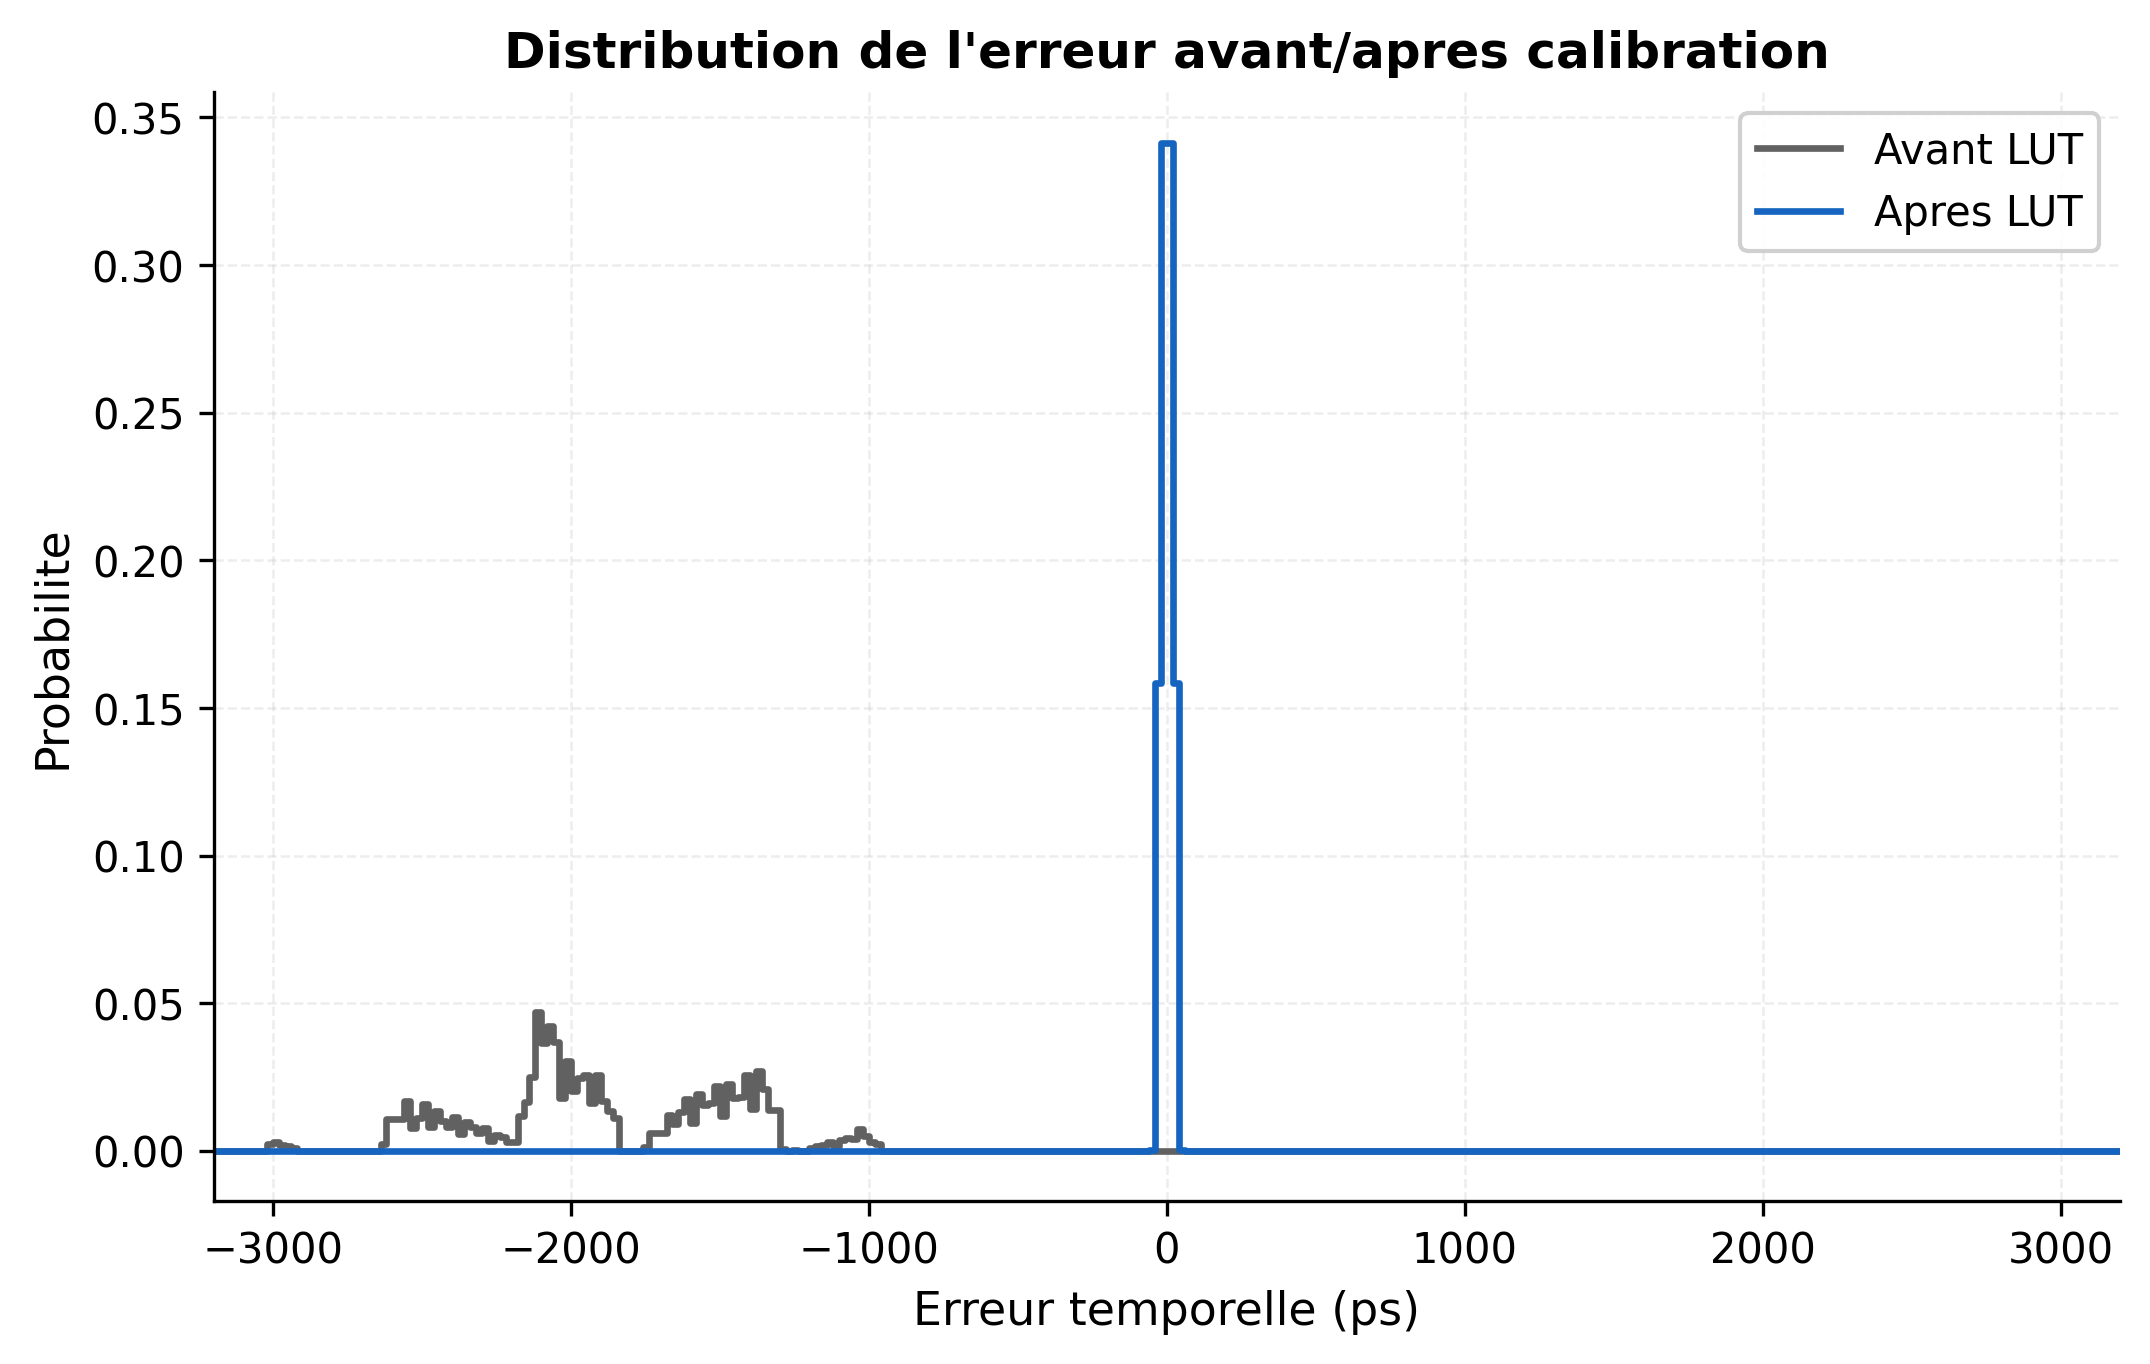
\includegraphics[width=\linewidth,height=0.66\textheight,keepaspectratio]{01_erreur_histogramme_pre_post_lut.png}
    \end{column}
    \begin{column}{0.29\textwidth}
      \vspace{0.42cm}
      \small
      \begin{itemize}
        \item Avant LUT : biais $\approx -1{,}9$ ns
        \item Erreur structurée par les observables bruts
        \item Après LUT : centrage proche de zéro
        \item Validation numérique pré-silicium
      \end{itemize}
    \end{column}
  \end{columns}

  \takeaway{La calibration corrige une structure systématique, elle ne masque pas une absence d'information.}
  \note{Objectif : corriger l'ambiguïté entre avant et après LUT. À dire : le biais d'environ -1,9 ns appartient à la mesure brute, avant correction ; après LUT, le centrage revient près de zéro. Transition : donner les chiffres de validation RTL/Xcelium.}
\end{frame}

% ---------------------------------------------------------------------------
\begin{frame}
  \frametitle{V. Linéarité observable des codes atteints}
  \lead{DNL et INL sont évaluées sur les codes réellement atteints, avec les codes absents explicitement reconnus.}

  \begin{columns}[T,totalwidth=0.98\textwidth]
    \begin{column}{0.66\textwidth}
      \centering
      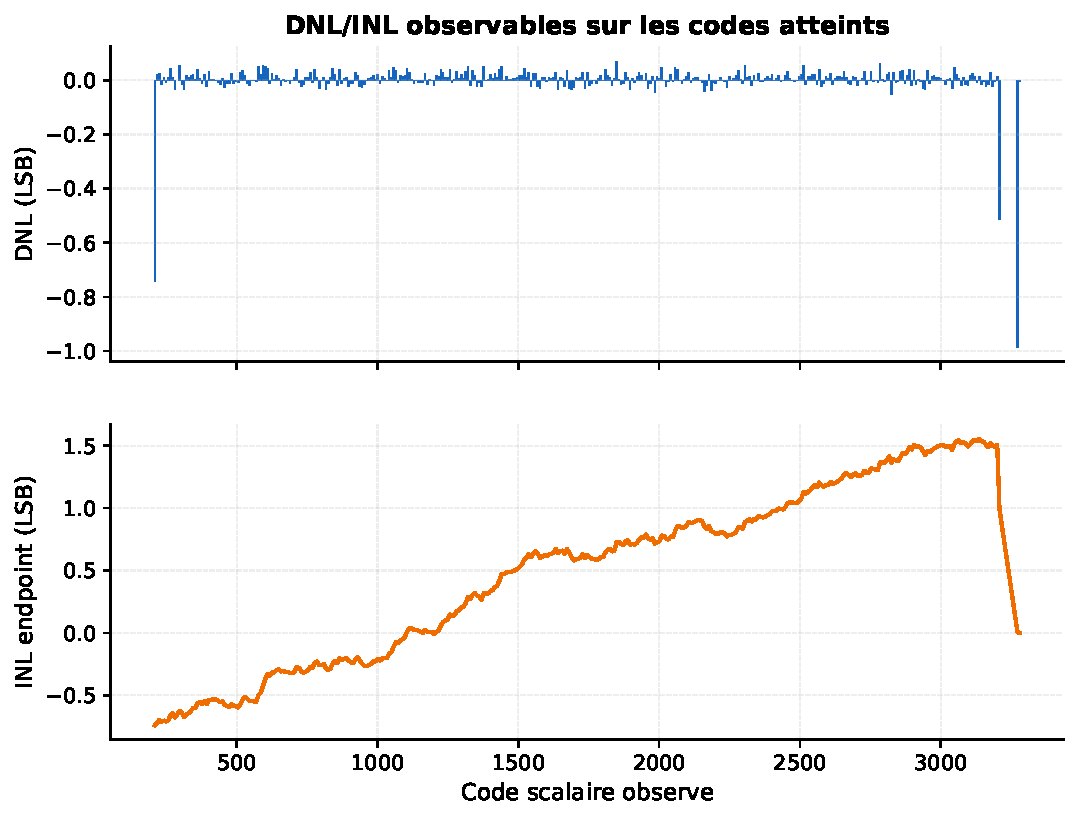
\includegraphics[width=\linewidth,height=0.68\textheight,keepaspectratio]{04_dnl_inl_observable.pdf}
    \end{column}
    \begin{column}{0.30\textwidth}
      \vspace{0.16cm}
      \small
      \begin{itemize}
        \item DNL pic $\approx 0{,}987$ LSB
        \item INL extrémité $\approx 1{,}553$ LSB
        \item Analyse limitée aux codes effectivement atteints
        \item Codes absents reconnus
        \item Non-uniformité cohérente avec la structure brute
      \end{itemize}
      \vspace{0.16cm}
      \smalltag{amber}{motive la LUT externe}
    \end{column}
  \end{columns}

  \takeaway{La linéarité observable confirme que la correction externe fait partie du flux de mesure.}
  \note{Objectif : placer DNL/INL dans la partie principale plutôt qu'en backup. À dire : les métriques ne supposent pas une répartition complète des codes ; elles portent sur les codes atteints, avec une non-uniformité cohérente avec la matrice brute et la nécessité de calibration. Transition : quantifier ensuite l'effet de la LUT sur l'erreur temporelle.}
\end{frame}

% ---------------------------------------------------------------------------
\begin{frame}
  \frametitle{Après LUT : RMSE = 18,56 ps}
  \lead{Résultat pré-silicium, calculé sur validation tenue hors apprentissage.}

  \begin{columns}[T,totalwidth=\textwidth]
    \begin{column}{0.58\textwidth}
      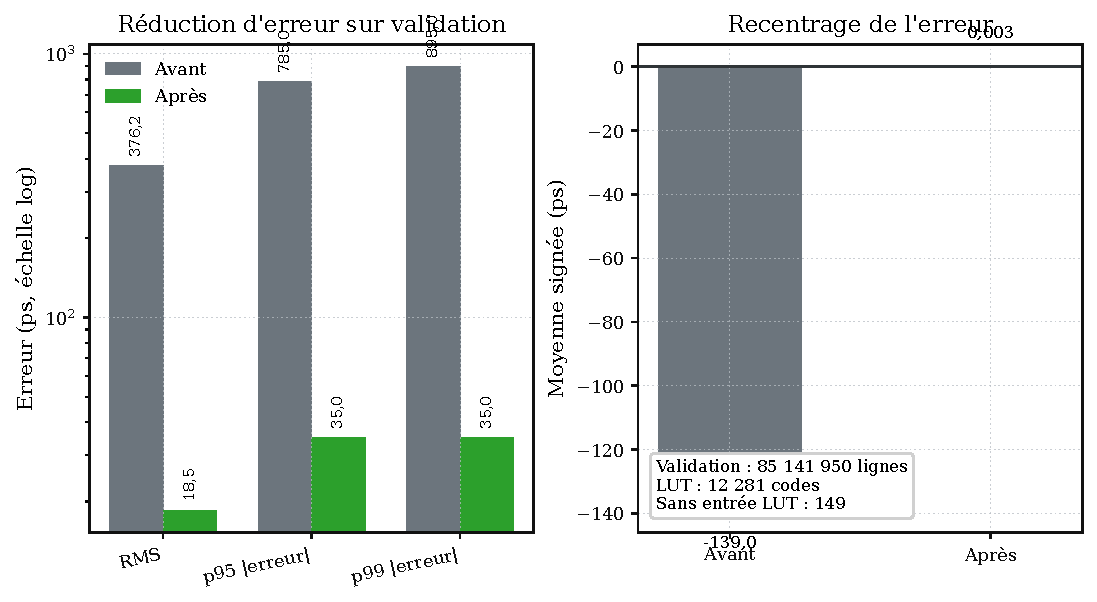
\includegraphics[width=\linewidth,height=0.66\textheight,keepaspectratio]{char_calibration_prepost_summary_report.pdf}
    \end{column}
    \begin{column}{0.38\textwidth}
      \metric{$\approx$1,94 ns}{RMSE brute}{amber}\\[0.12cm]
      \metric{18,56 ps}{RMSE après LUT}{navy}\\[0.12cm]
      \metric{38,99 ps}{P99 erreur absolue}{navy}
    \end{column}
  \end{columns}

  \vspace{-0.02cm}
  \begin{center}
    \smalltag{amber}{RTL/Xcelium -- validation hors apprentissage -- pré-silicium}
  \end{center}

  \takeaway{Ce chiffre valide le flux d'observables et de correction ; il reste une validation RTL/Xcelium pré-silicium.}
  \note{Objectif : citer le résultat principal avec exactitude. À dire : RMSE brute environ 1,94 ns, RMSE après LUT 18,56 ps, P99 absolu 38,99 ps, sur validation hors apprentissage. Transition : présenter le moyennage comme gain statistique séparé.}
\end{frame}

% ---------------------------------------------------------------------------
\begin{frame}
  \frametitle{Moyennage post-LUT : gain statistique}
  \lead{Analyse statistique après correction LUT, pas performance par événement unique.}

  \begin{columns}[T,totalwidth=\textwidth]
    \begin{column}{0.62\textwidth}
      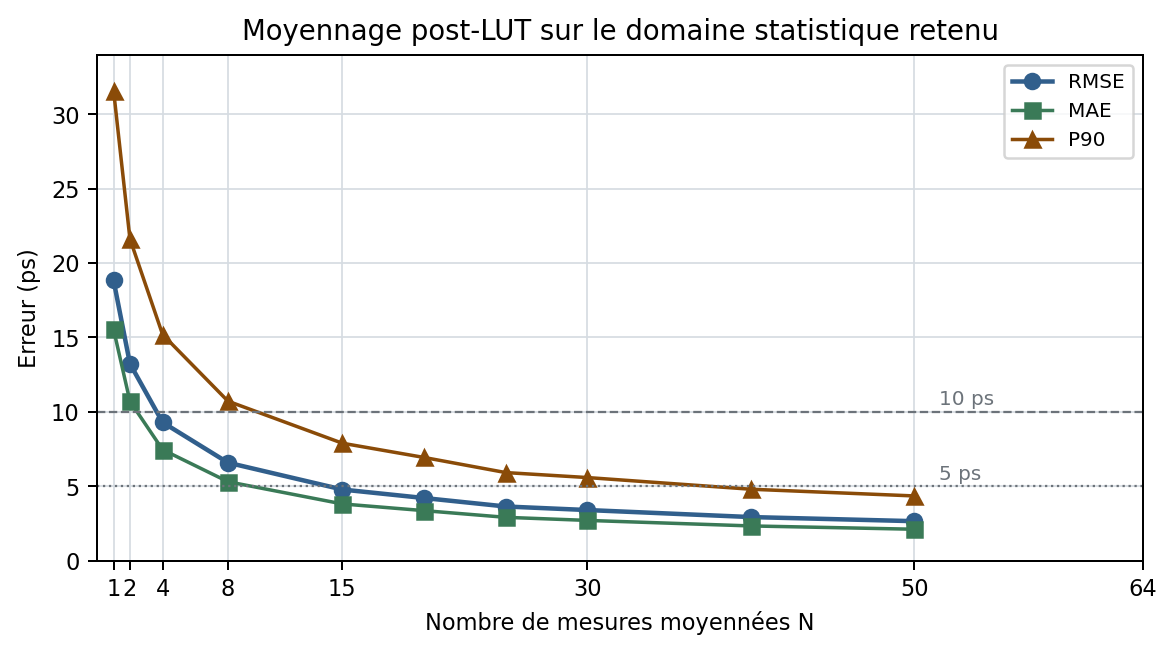
\includegraphics[width=\linewidth,height=0.72\textheight,keepaspectratio]{03_rmse_vs_moyennage_limited.png}
    \end{column}
    \begin{column}{0.34\textwidth}
      \begin{itemize}
        \item $N=1 \rightarrow 18{,}82$ ps
        \item $N=4 \rightarrow 9{,}28$ ps
        \item $N=15 \rightarrow 4{,}77$ ps
      \end{itemize}
      \vspace{0.25cm}
      \smalltag{amber}{prudence : pas par événement unique}
    \end{column}
  \end{columns}

  \takeaway{Le gain par moyennage est utile, mais doit rester présenté avec son domaine de validité.}
  \note{Objectif : éviter de survendre le moyennage. À dire : N=4 donne 9,28 ps et N=15 donne 4,77 ps dans l'analyse post-LUT, mais ce n'est pas une performance mono-événement. Transition : revenir aux limites physiques qui restent décisives.}
\end{frame}

\section[Limites]{Limites et perspectives}

\chaptertransition{VI}{Limites et perspectives}{Clarifier ce que la simulation RTL valide, puis ouvrir vers le signoff physique.}

% ---------------------------------------------------------------------------
\begin{frame}
  \frametitle{La performance finale reste physique}
  \lead{Le prochain verrou n'est plus seulement RTL : il est CDC, STA, layout, jitter et silicium.}

  \begin{center}
  \begin{tikzpicture}[
    s/.style={basebox,minimum width=2.0cm,minimum height=0.8cm},
    w/.style={warnbox,minimum width=2.0cm,minimum height=0.8cm}
  ]
    \node[s,draw=navy!55,fill=navy!4] (rtl) {RTL};
    \node[s,right=0.28cm of rtl] (cdc) {CDC};
    \node[s,right=0.28cm of cdc] (sta) {STA};
    \node[s,right=0.28cm of sta] (pnr) {PnR};
    \node[s,right=0.28cm of pnr] (post) {Post-layout};
    \node[w,right=0.28cm of post] (sil) {Silicium};
    \foreach \a/\b in {rtl/cdc,cdc/sta,sta/pnr,pnr/post,post/sil}
      \draw[softarrow] (\a) -- (\b);
  \end{tikzpicture}
  \end{center}

  \begin{columns}[T,totalwidth=\textwidth]
    \begin{column}{0.48\textwidth}
      \begin{itemize}
        \item Oscillateurs réels
        \item Setup / hold / skew
        \item Jitter et variations PVT
      \end{itemize}
    \end{column}
    \begin{column}{0.48\textwidth}
      \begin{itemize}
        \item Revue CDC formelle
        \item Simulations post-layout
        \item Corrélation mesures silicium
      \end{itemize}
    \end{column}
  \end{columns}

  \takeaway{La conclusion honnête : le numérique est cohérent, la performance finale reste à démontrer physiquement.}
  \note{Objectif : poser clairement la limite avant la conclusion. À dire : CDC, STA, PnR, extraction, jitter, PVT et silicium restent les étapes qui transformeront le contrat numérique en performance physique. Transition : résumer en trois messages.}
\end{frame}

% ---------------------------------------------------------------------------
\begin{frame}
  \frametitle{Trois messages à retenir}
  \lead{La conclusion doit être simple, défendable et honnête devant le jury.}

  \begin{center}
  \begin{tikzpicture}[
    msg/.style={basebox,minimum width=8.8cm,minimum height=0.95cm,text width=8.2cm,align=left}
  ]
    \node[msg,draw=navy!55,fill=navy!4] (a) {\bfseries 1. Architecture : \normalfont Vernier multiphase rendu intégrable dans SPADMIC.};
    \node[msg,below=0.25cm of a] (b) {\bfseries 2. Preuve numérique : \normalfont protocole vérifié et calibration efficace en RTL/Xcelium.};
    \node[msg,draw=amber!65,fill=amberSoft,below=0.25cm of b] (c) {\bfseries 3. Limite : \normalfont performance physique à confirmer par post-layout et silicium.};
  \end{tikzpicture}
  \end{center}

  \takeaway{Le récit est ambitieux sur l'ingénierie numérique, prudent sur la performance physique.}
  \note{Objectif : fermer sans ouvrir un nouveau sujet. À dire : architecture intégrable, preuve numérique pré-silicium, limite physique assumée. Transition : remercier et basculer vers les questions.}
\end{frame}

% ---------------------------------------------------------------------------
\begin{frame}
  \frametitle{Merci pour votre attention}
  \lead{Questions}

  \vspace{0.4cm}
  \begin{center}
    {\Huge\bfseries\color{navy2}Questions ?}\\[0.65cm]
    \begin{tabular}{@{}ll@{}}
      Karim SABRA & CPE Lyon -- IP2I / CNRS\\
      Encadrant IP2I & Edouard Bechetoille\\
      Encadrant école & Abdelbassat Massouri\\
      Sujet & SPADMIC
    \end{tabular}
  \end{center}
  \note{Objectif : laisser une slide claire pour les échanges. À dire : remercier le jury, les encadrants et l'équipe. Transition : utiliser les backups selon la question posée.}
\end{frame}

% ---------------------------------------------------------------------------
% Backup slides
% ---------------------------------------------------------------------------
\appendix
\section{Backup}

\begin{frame}[noframenumbering]
  \frametitle{Backup -- Détail du Vernier}
  \lead{La résolution élémentaire vient de la différence entre deux délais proches.}
  \begin{center}
    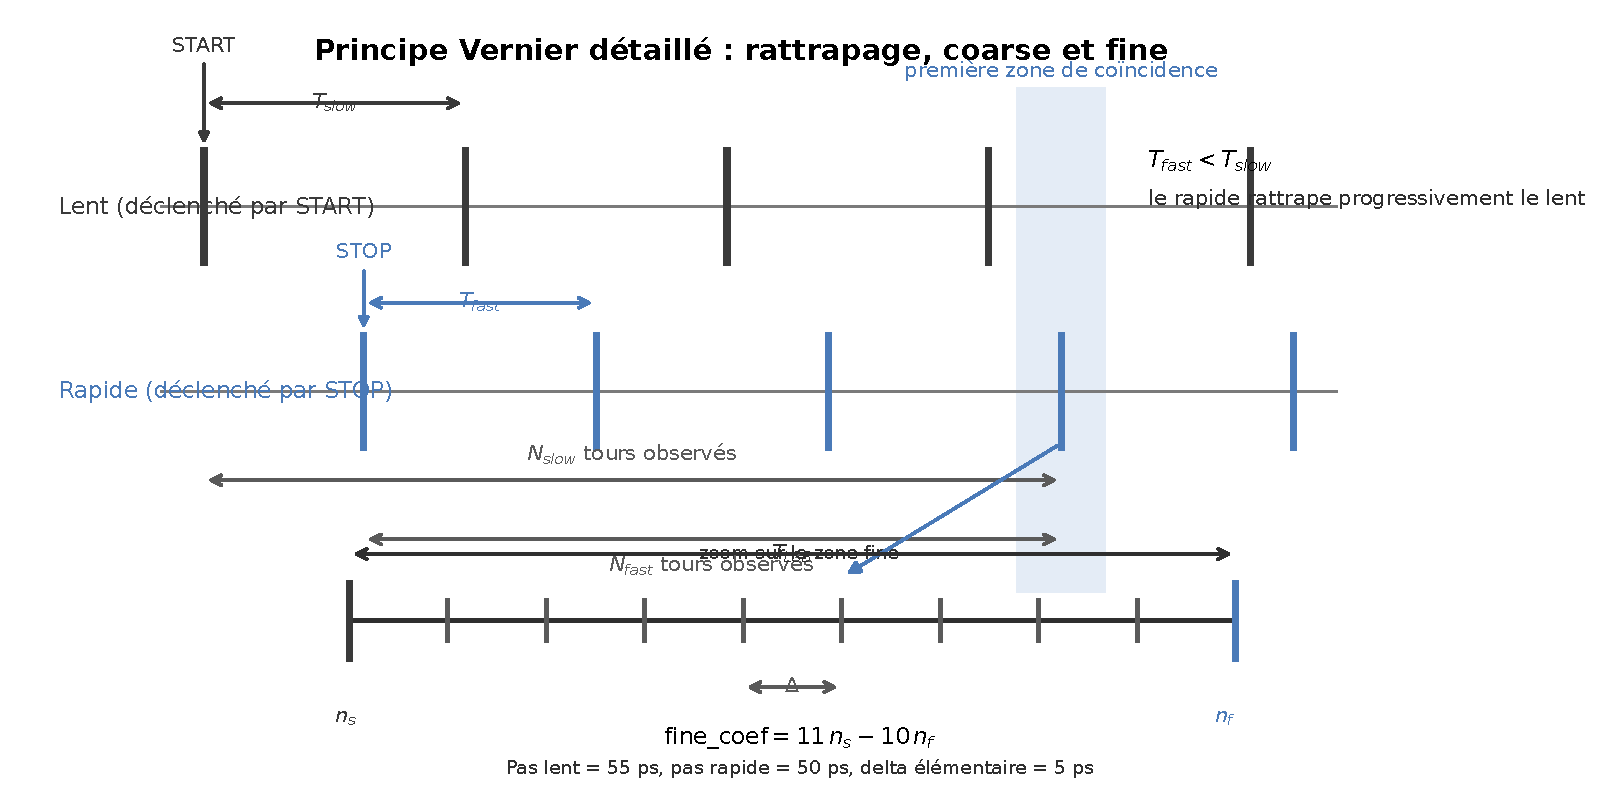
\includegraphics[width=0.92\textwidth,height=0.70\textheight,keepaspectratio]{vernier_timing_principle.pdf}
  \end{center}
  \takeaway{$T_{\mathrm{LSB}} = T_{\mathrm{slow}} - T_{\mathrm{fast}}$, avec prudence sur l'implémentation physique réelle.}
  \note{Question traitée : revenir au rattrapage Vernier si le jury veut le détail physique. Réponse clé : le pas différentiel est conceptuel et doit être confronté aux délais réels post-layout.}
\end{frame}

\begin{frame}[noframenumbering]
  \frametitle{Backup -- Multiphase versus moyennage}
  \lead{Deux notions différentes : enrichir une conversion, puis moyenner plusieurs estimations corrigées.}
  \begin{columns}[T,totalwidth=\textwidth]
    \begin{column}{0.54\textwidth}
      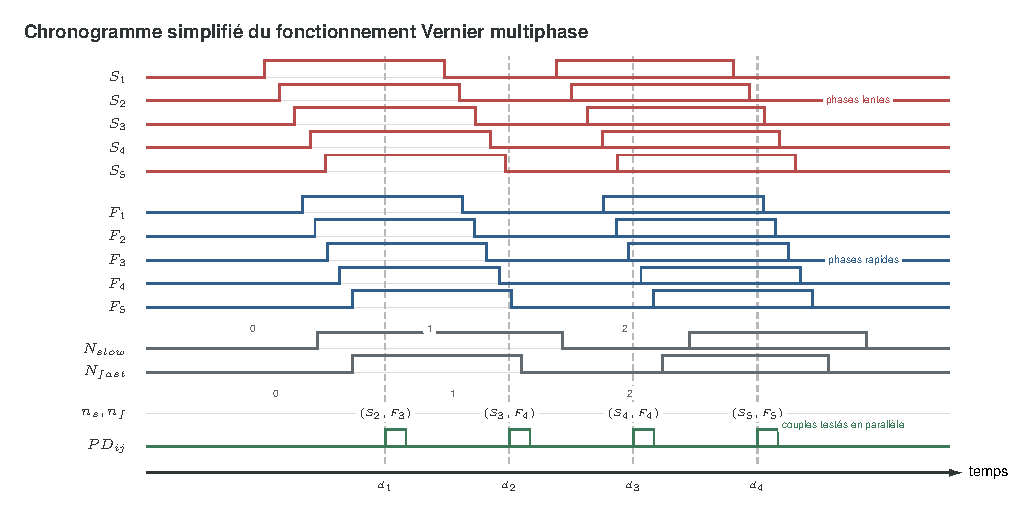
\includegraphics[width=\linewidth,height=0.62\textheight,keepaspectratio]{vernier_multiphase_timing.pdf}
    \end{column}
    \begin{column}{0.42\textwidth}
      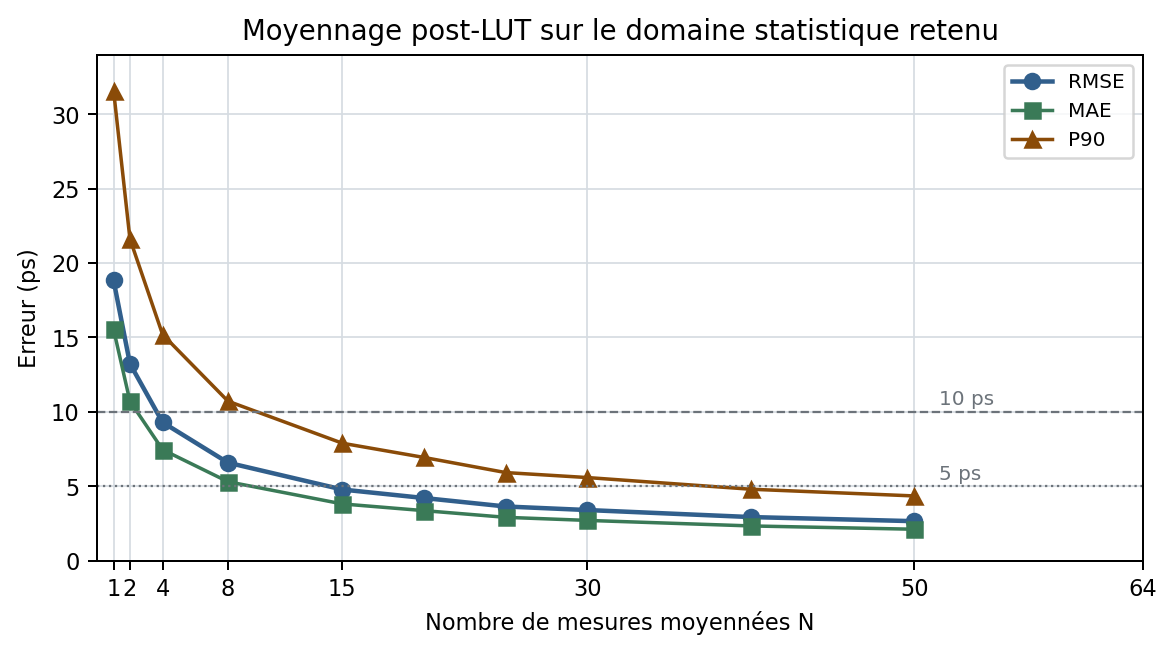
\includegraphics[width=\linewidth,height=0.62\textheight,keepaspectratio]{03_rmse_vs_moyennage_limited.png}
    \end{column}
  \end{columns}
  \vspace{-0.16cm}
  \begin{center}
    \smalltag{navy}{multiphase : une conversion}\hspace{0.35cm}
    \smalltag{amber}{moyennage : plusieurs mesures corrigées}
  \end{center}
  \takeaway{Le multiphase est architectural ; le moyennage est statistique.}
  \note{Question traitée : éviter la confusion entre plusieurs phases dans une conversion et plusieurs mesures moyennées après LUT. Réponse clé : les deux mécanismes n'agissent pas au même endroit de la chaîne.}
\end{frame}

\begin{frame}[noframenumbering]
  \frametitle{Backup -- Pourquoi trois axes MPTDC ?}
  \lead{Les voies temporelles sont coordonnées avec la logique de lecture spatiale de SPADMIC.}
  \begin{center}
    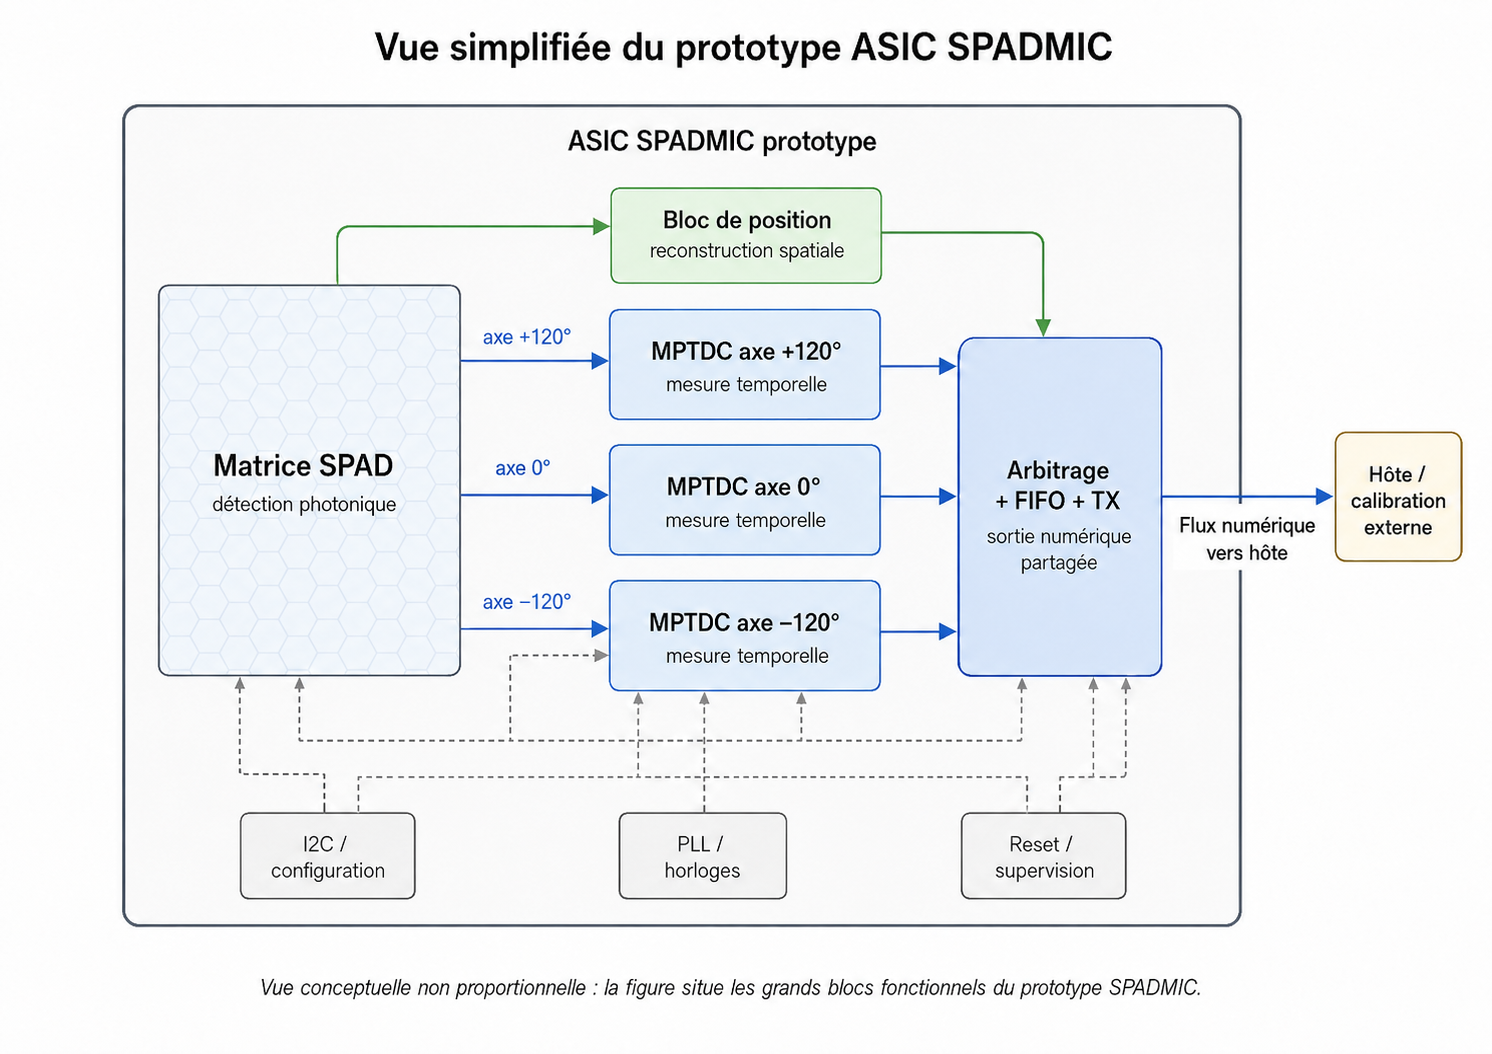
\includegraphics[width=0.82\textwidth,height=0.50\textheight,keepaspectratio]{spadmic_mind_model.png}
  \end{center}
  \takeaway{Ce ne sont pas trois canaux indépendants abstraits : ils participent à la lecture tri-axis du prototype.}
  \note{Question traitée : pourquoi trois voies temporelles. Réponse clé : elles suivent la logique de projections tri-axis de SPADMIC et partagent ensuite la chaîne de sortie.}
\end{frame}

\begin{frame}[noframenumbering]
  \frametitle{Backup -- Paquet et clé LUT}
  \lead{La correction hôte utilise des champs observables, pas seulement un code temporel brut.}
  \begin{center}
    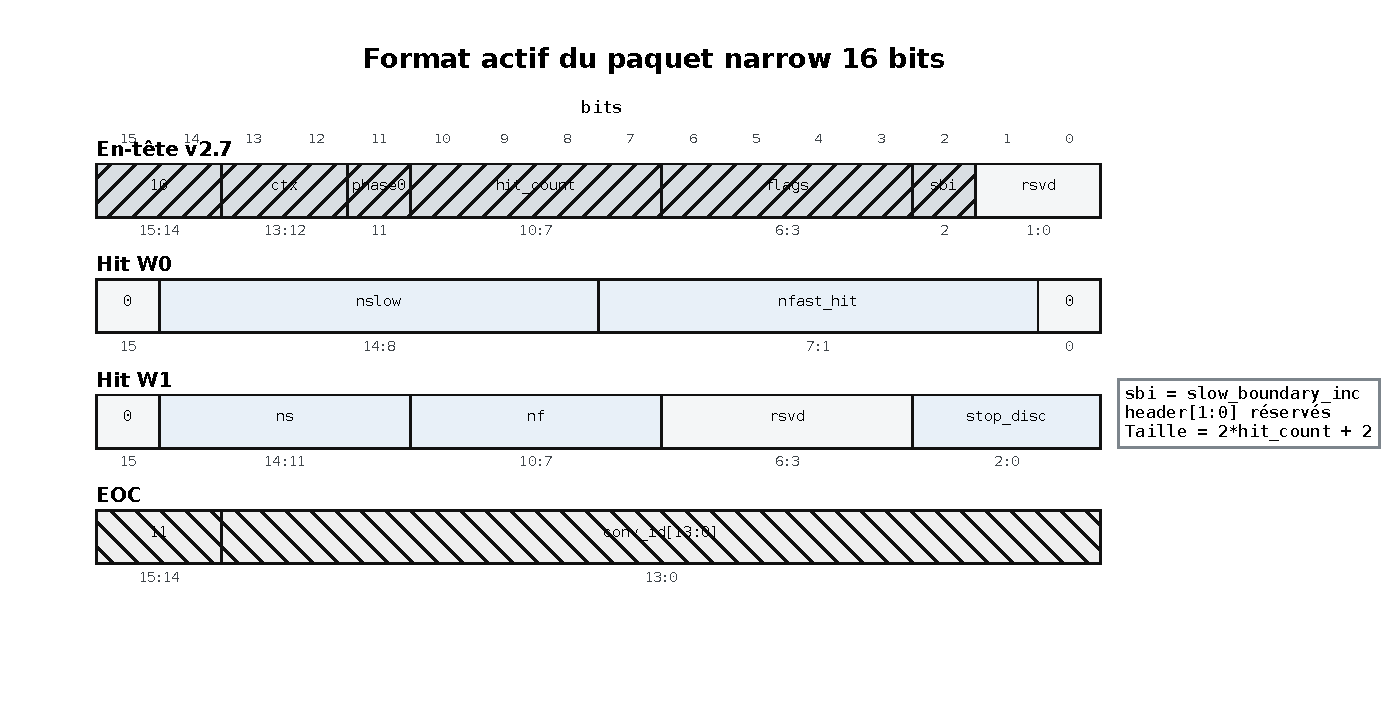
\includegraphics[width=0.98\textwidth,height=0.63\textheight,keepaspectratio]{packet_format_v27.pdf}
  \end{center}
  \vspace{-0.10cm}
  \begin{center}
    \smalltag{navy}{$n_{\mathrm{fast}}/n_{\mathrm{slow}}$}\hspace{0.25cm}
    \smalltag{navy}{indices de phase}\hspace{0.25cm}
    \smalltag{navy}{hit / STOP}\hspace{0.25cm}
    \smalltag{amber}{clé LUT hôte}
  \end{center}
  \takeaway{La trame est pensée pour rendre la calibration possible après acquisition.}
  \note{Question traitée : quelles informations alimentent la LUT. Réponse clé : compteurs, phases, hit, statuts et métadonnées construisent une clé d'observables côté hôte.}
\end{frame}

\begin{frame}[noframenumbering]
  \frametitle{Backup -- DNL/INL sur codes observés}
  \lead{Ces chiffres ne décrivent pas toute la répartition théorique, seulement les codes effectivement atteints.}
  \begin{columns}[T,totalwidth=\textwidth]
    \begin{column}{0.62\textwidth}
      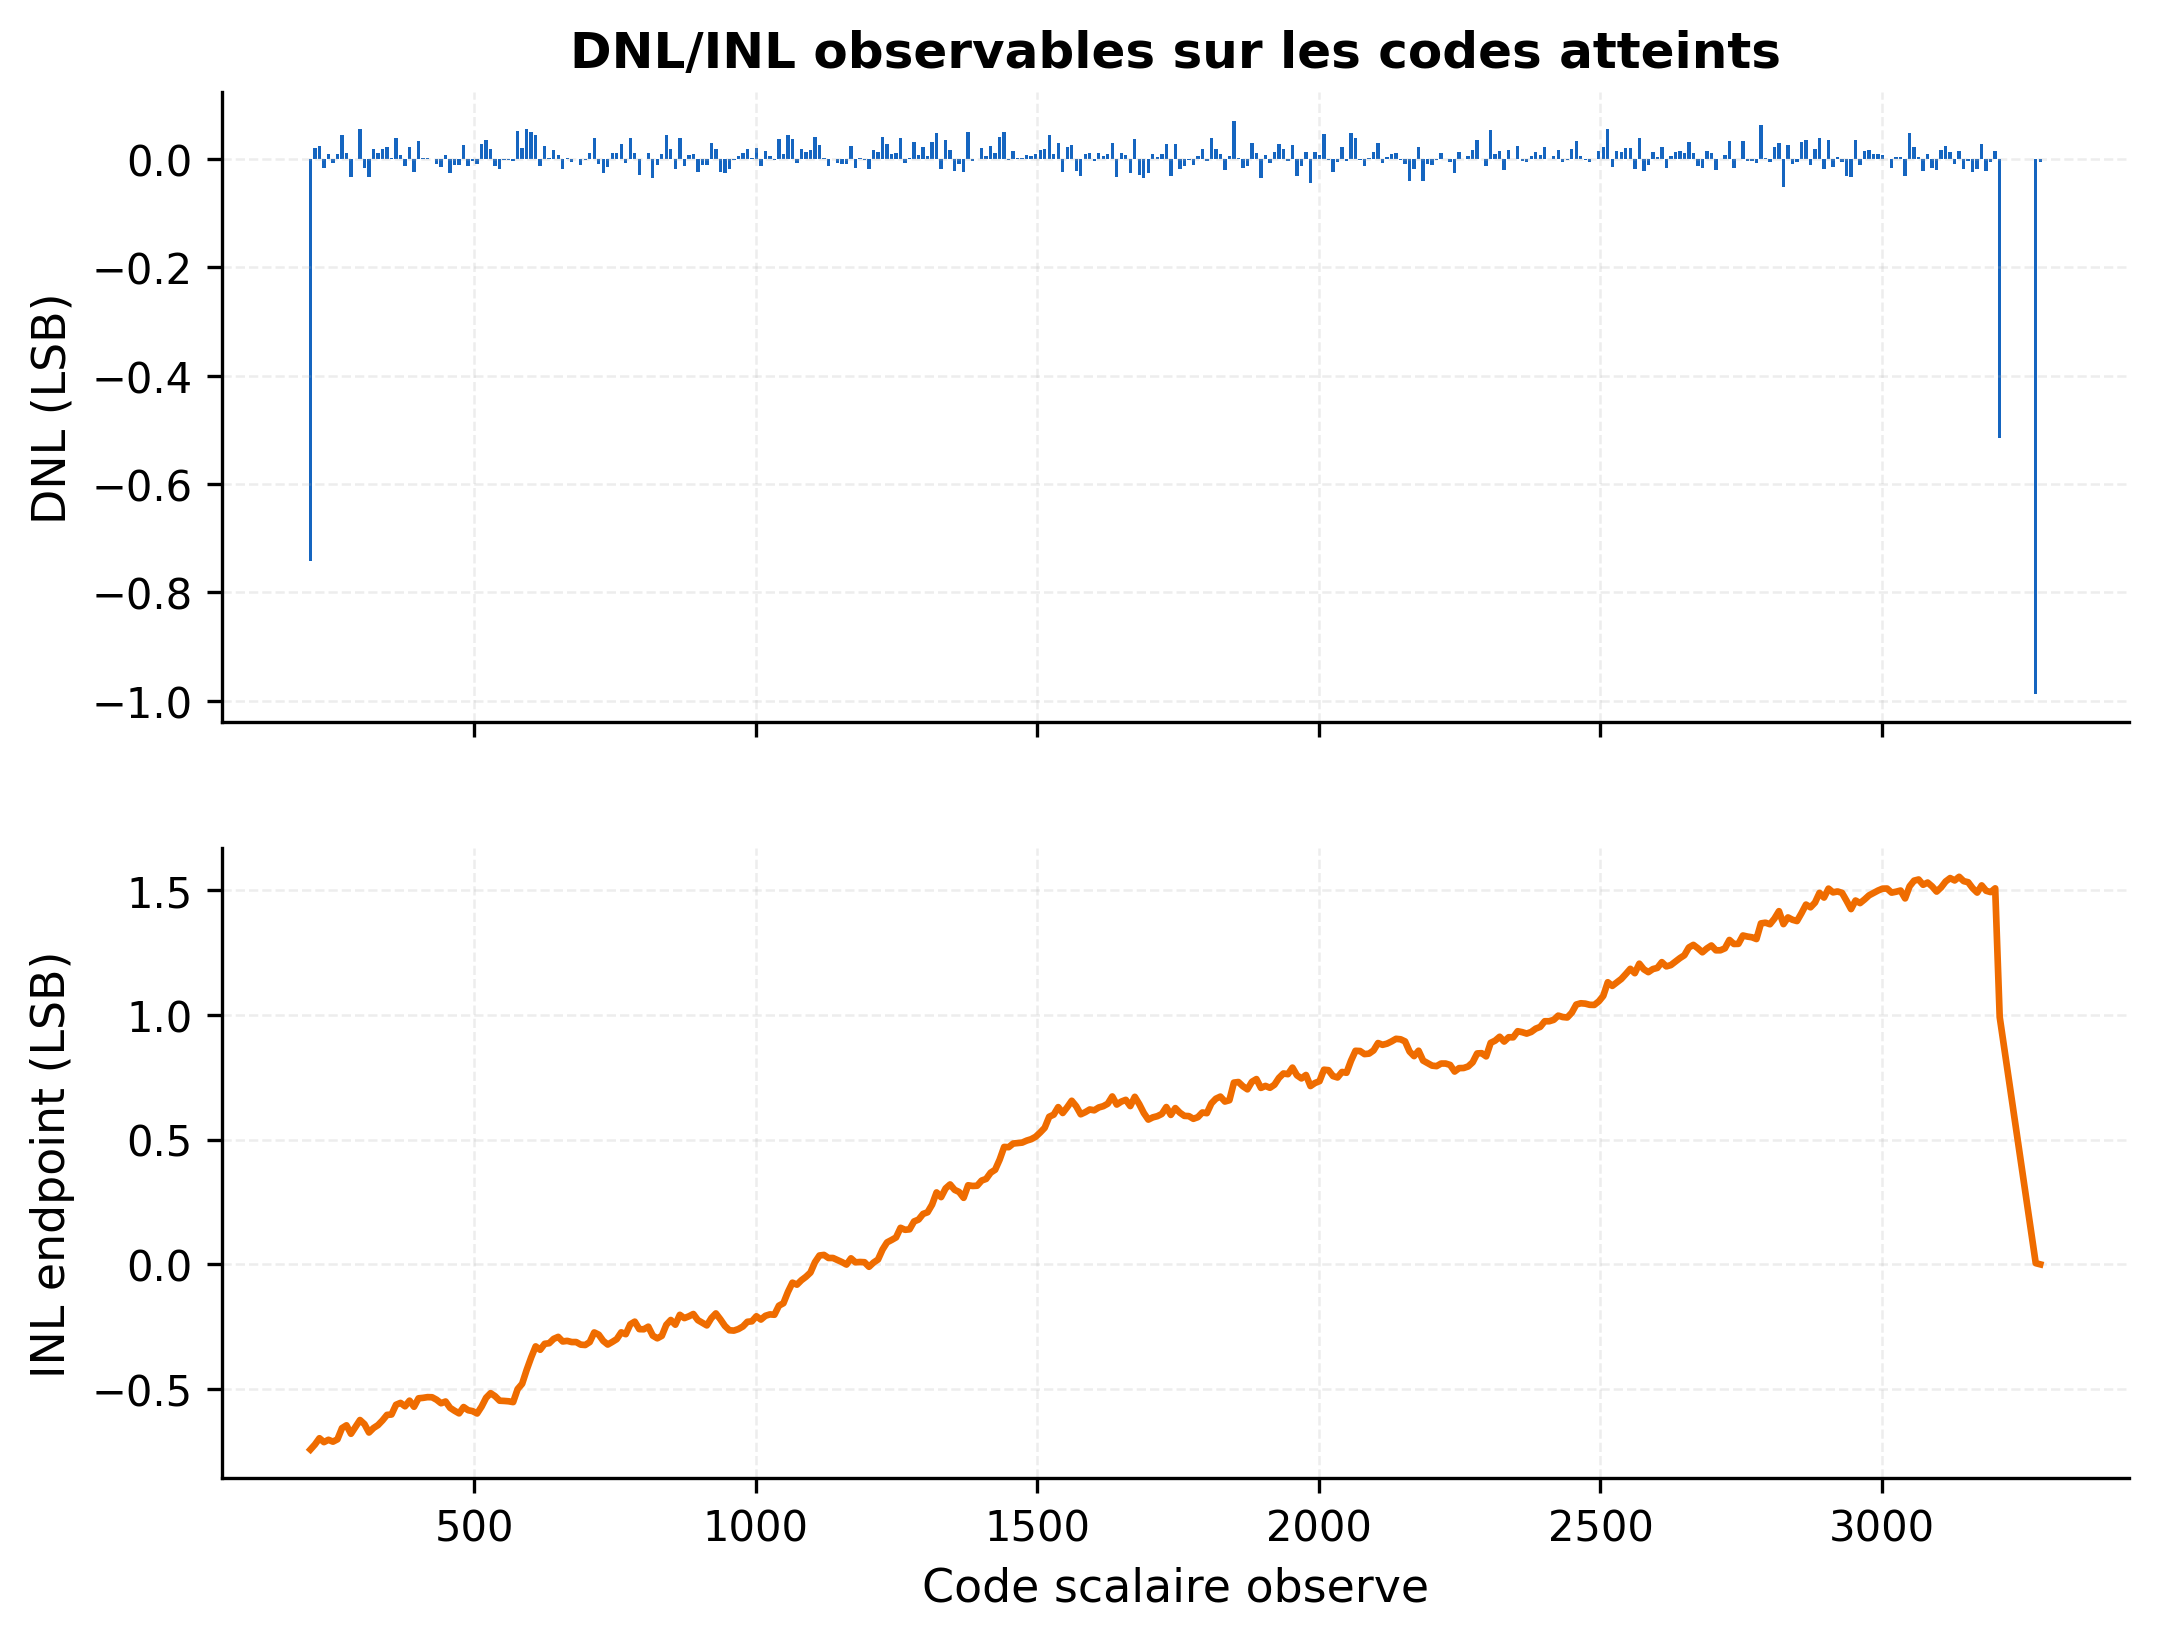
\includegraphics[width=\linewidth,height=0.60\textheight,keepaspectratio]{04_dnl_inl_observable.png}
    \end{column}
    \begin{column}{0.34\textwidth}
      \begin{itemize}
        \item DNL pic : $0{,}987$ LSB
        \item INL extrémité : $1{,}553$ LSB
        \item Codes manquants explicitement reconnus
      \end{itemize}
    \end{column}
  \end{columns}
  \takeaway{La linéarité est défendue sur le domaine observé, pas comme propriété universelle de la matrice complète.}
  \note{Question traitée : existence de codes manquants et validité DNL/INL. Réponse clé : les métriques sont sur les codes observés, pas sur une répartition théorique supposée pleine.}
\end{frame}

\begin{frame}[noframenumbering]
  \frametitle{Backup -- Validation hors apprentissage}
  \lead{La LUT est construite et évaluée sur des ensembles séparés.}
  \begin{center}
    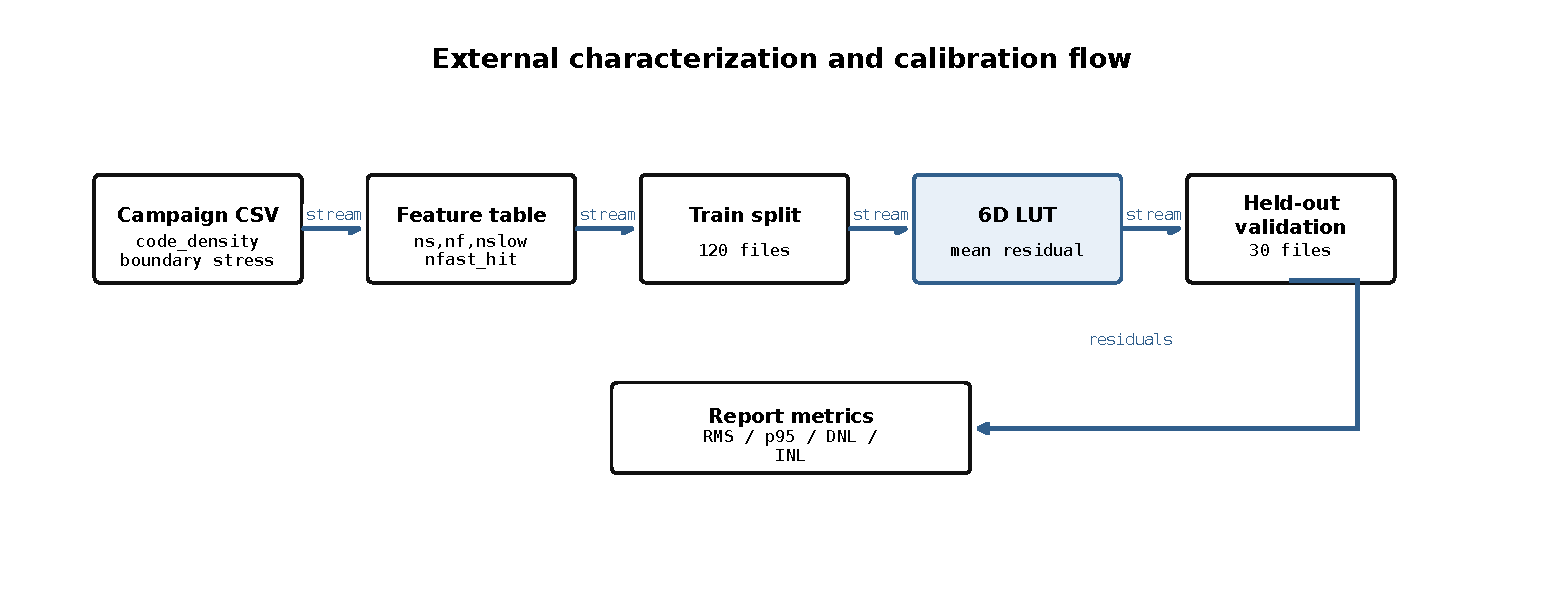
\includegraphics[width=0.94\textwidth,height=0.62\textheight,keepaspectratio]{calibration_flow.pdf}
  \end{center}
  \vspace{-0.10cm}
  \begin{center}
    \smalltag{navy}{split train}\hspace{0.35cm}
    \smalltag{navy}{LUT figée}\hspace{0.35cm}
    \smalltag{amber}{validation fresh}
  \end{center}
  \takeaway{Les 18,56 ps sont une métrique de validation RTL/Xcelium hors apprentissage.}
  \note{Question traitée : risque d'apprentissage de la LUT. Réponse clé : la LUT est figée avant validation et la métrique est rapportée hors apprentissage.}
\end{frame}

\begin{frame}[noframenumbering]
  \frametitle{Backup -- Rétropression et saturation}
  \lead{Deux contextes réduisent le temps mort, mais ne rendent pas le débit infini.}
  \begin{center}
    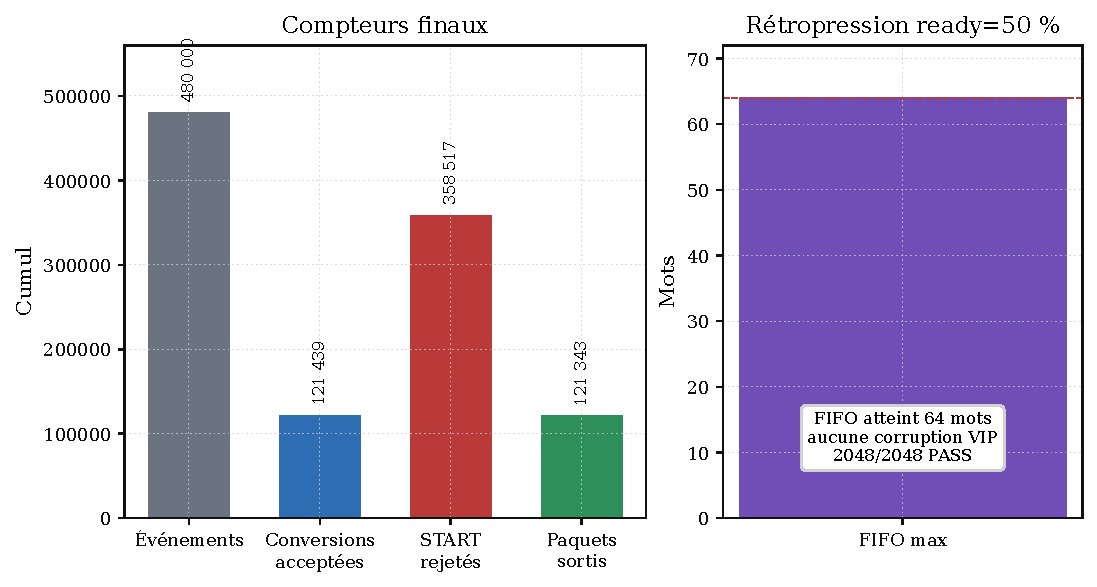
\includegraphics[width=0.84\textwidth,height=0.68\textheight,keepaspectratio]{char_throughput_counters_report.pdf}
  \end{center}
  \vspace{-0.08cm}
  \begin{center}
    \smalltag{navy}{ready/valid}\hspace{0.35cm}
    \smalltag{navy}{FIFO 64 mots}\hspace{0.35cm}
    \smalltag{amber}{débit borné}
  \end{center}
  \takeaway{La saturation est une limite système à rendre visible, pas à cacher.}
  \note{Question traitée : débit et blocage aval. Réponse clé : deux contextes aident, mais ready/valid et saturation restent à gérer comme limites système.}
\end{frame}

\begin{frame}[noframenumbering]
  \frametitle{Backup -- Watchdogs et absence de STOP}
  \lead{Les scénarios incomplets doivent aboutir à un état observable et récupérable.}
  \begin{center}
    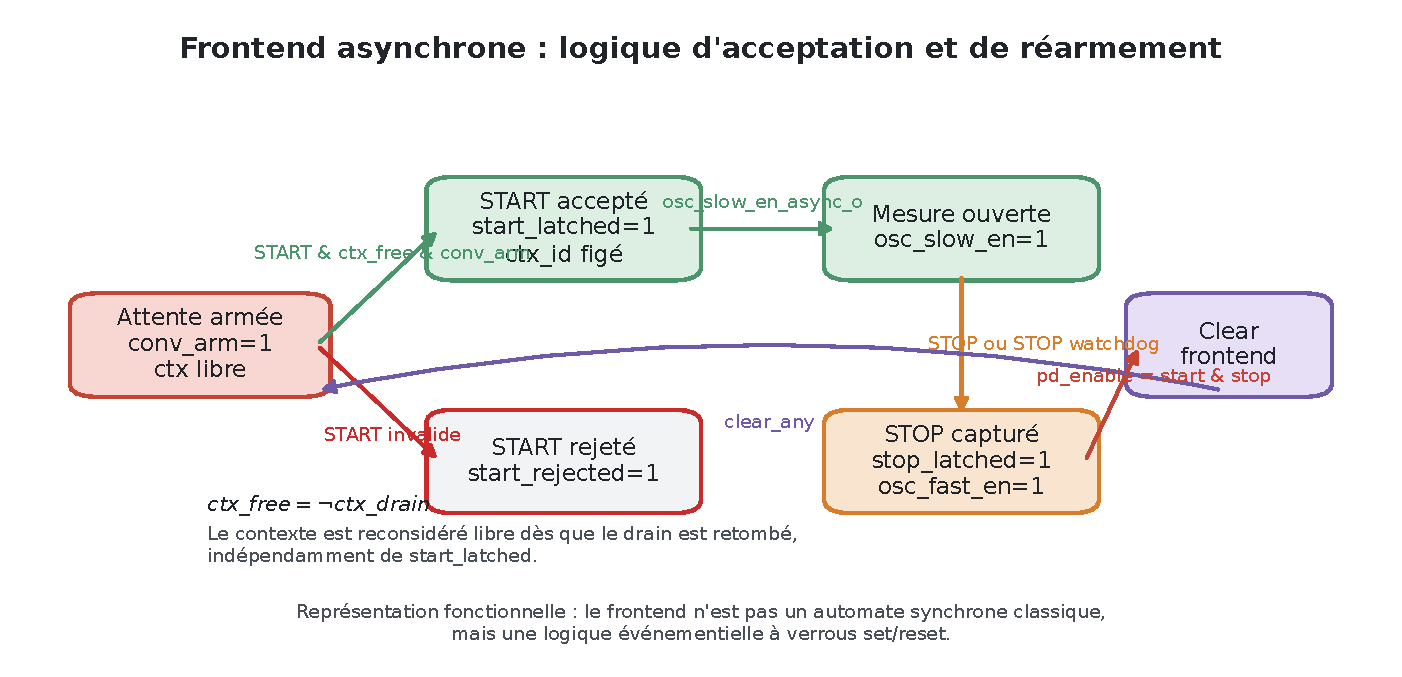
\includegraphics[width=0.88\textwidth,height=0.66\textheight,keepaspectratio]{async_frontend_fsm.pdf}
  \end{center}
  \vspace{-0.08cm}
  \begin{center}
    \smalltag{navy}{START}\hspace{0.35cm}
    \smalltag{amber}{timeout}\hspace{0.35cm}
    \smalltag{navy}{CLEAR}
  \end{center}
  \takeaway{Un cas d'erreur maîtrisé est préférable à une conversion bloquée ou silencieuse.}
  \note{Question traitée : que se passe-t-il si STOP n'arrive pas. Réponse clé : le watchdog doit conduire à un statut exporté et à une récupération contrôlée.}
\end{frame}

\begin{frame}[noframenumbering]
  \frametitle{Backup -- CDC et compteurs Gray}
  \lead{La stratégie réduit le risque de mots incohérents, mais n'est pas un signoff CDC formel.}
  \begin{center}
    
\includegraphics[width=0.98\textwidth,height=0.66\textheight,keepaspectratio]{clock_domain_diagram.pdf}
  \end{center}
  \vspace{-0.08cm}
  \begin{center}
    \smalltag{navy}{compteurs Gray}\hspace{0.35cm}
    \smalltag{navy}{snapshot stable}\hspace{0.35cm}
    \smalltag{amber}{revue CDC à finaliser}
  \end{center}
  \takeaway{Au niveau RTL, on réduit et observe le risque ; au niveau physique, il faut le signer.}
  \note{Question traitée : robustesse CDC et compteurs Gray. Réponse clé : le RTL réduit le risque de mots incohérents, mais une revue CDC formelle reste nécessaire.}
\end{frame}

\begin{frame}[noframenumbering]
  \frametitle{Backup -- Roadmap de signoff physique}
  \lead{La suite naturelle est une boucle de corrélation entre simulations physiques et mesures.}
  \begin{center}
  \resizebox{0.94\textwidth}{!}{%
  \begin{tikzpicture}[
    s/.style={basebox,minimum width=2.15cm,minimum height=0.82cm},
    w/.style={warnbox,minimum width=2.15cm,minimum height=0.82cm}
  ]
    \node[s,draw=navy!55,fill=navy!4] (rtl) {RTL};
    \node[s,right=0.22cm of rtl] (syn) {Synthèse};
    \node[s,right=0.22cm of syn] (sta) {STA / CDC};
    \node[s,right=0.22cm of sta] (pnr) {PnR};
    \node[s,right=0.22cm of pnr] (post) {Post-layout};
    \node[w,right=0.22cm of post] (sil) {Silicium};
    \foreach \a/\b in {rtl/syn,syn/sta,sta/pnr,pnr/post,post/sil}
      \draw[softarrow] (\a) -- (\b);
  \end{tikzpicture}%
  }
  \end{center}
  \takeaway{Le support doit finir sur cette feuille de route, pas sur une promesse de performance finale.}
  \note{Question traitée : prochaines étapes pour transformer le résultat RTL en circuit. Réponse clé : synthèse, STA/CDC, PnR, post-layout puis corrélation silicium.}
\end{frame}

\begin{frame}[noframenumbering]
  \frametitle{Backup -- Reset global vs clear de conversion}
  \lead{Reset et clear appartiennent à deux temps différents du protocole.}

  \begin{center}
    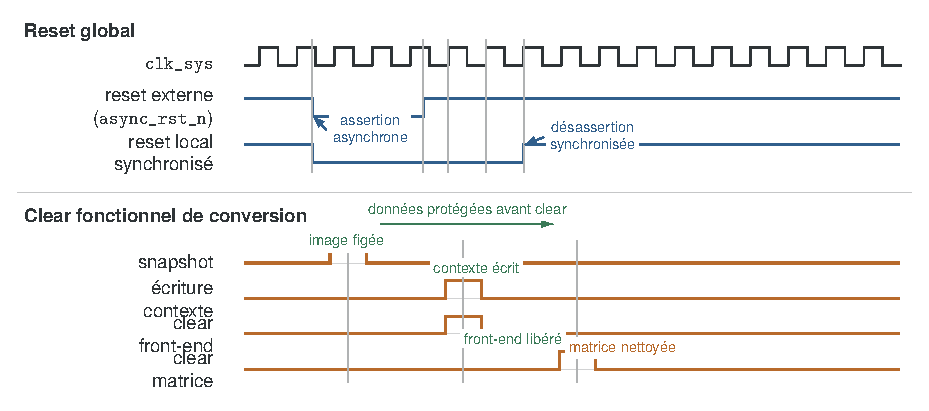
\includegraphics[width=0.98\textwidth,height=0.67\textheight,keepaspectratio]{reset_clear_sequence.pdf}
  \end{center}
  \vspace{-0.08cm}
  \begin{center}
    \smalltag{navy}{reset global}\hspace{0.35cm}
    \smalltag{navy}{snapshot / contexte}\hspace{0.35cm}
    \smalltag{amber}{clear après image figée}
  \end{center}

  \takeaway{Le reset sécurise l'état global ; le clear nettoie seulement après protection de l'image utile.}
  \note{Question traitée : différence entre reset et clear. Réponse clé : le reset initialise le système, tandis que le clear est une étape contrôlée de fin de conversion après snapshot et contexte.}
\end{frame}

\begin{frame}[noframenumbering]
  \frametitle{Backup -- Questions probables du jury}
  \lead{Cette slide sert de carte mentale pour orienter les réponses vers les backups adaptés.}

  \begin{columns}[T,totalwidth=\textwidth]
    \begin{column}{0.48\textwidth}
      \begin{itemize}
        \item Pourquoi ne pas utiliser directement l'horloge système ?
        \item Que transporte vraiment la trame 16 bit ?
        \item Pourquoi l'erreur brute est-elle aussi biaisée ?
        \item Le moyennage promet-il moins de 5 ps par hit ?
      \end{itemize}
    \end{column}
    \begin{column}{0.48\textwidth}
      \begin{itemize}
        \item Que prouvent les 18,56 ps ?
        \item Où sont les risques CDC restants ?
        \item Que manque-t-il avant les mesures silicium ?
        \item Pourquoi trois axes MPTDC dans SPADMIC ?
      \end{itemize}
    \end{column}
  \end{columns}

  \takeaway{Répondre en revenant toujours au contrat : observables, correction, portée pré-silicium, limites physiques.}
  \note{Question traitée : préparer la navigation en Q&A. Réponse clé : choisir le backup correspondant et garder la frontière RTL/Xcelium pré-silicium visible.}
\end{frame}

\end{document}
